% Created by tikzDevice version 0.12.3 on 2020-03-20 23:21:31
% !TEX encoding = UTF-8 Unicode
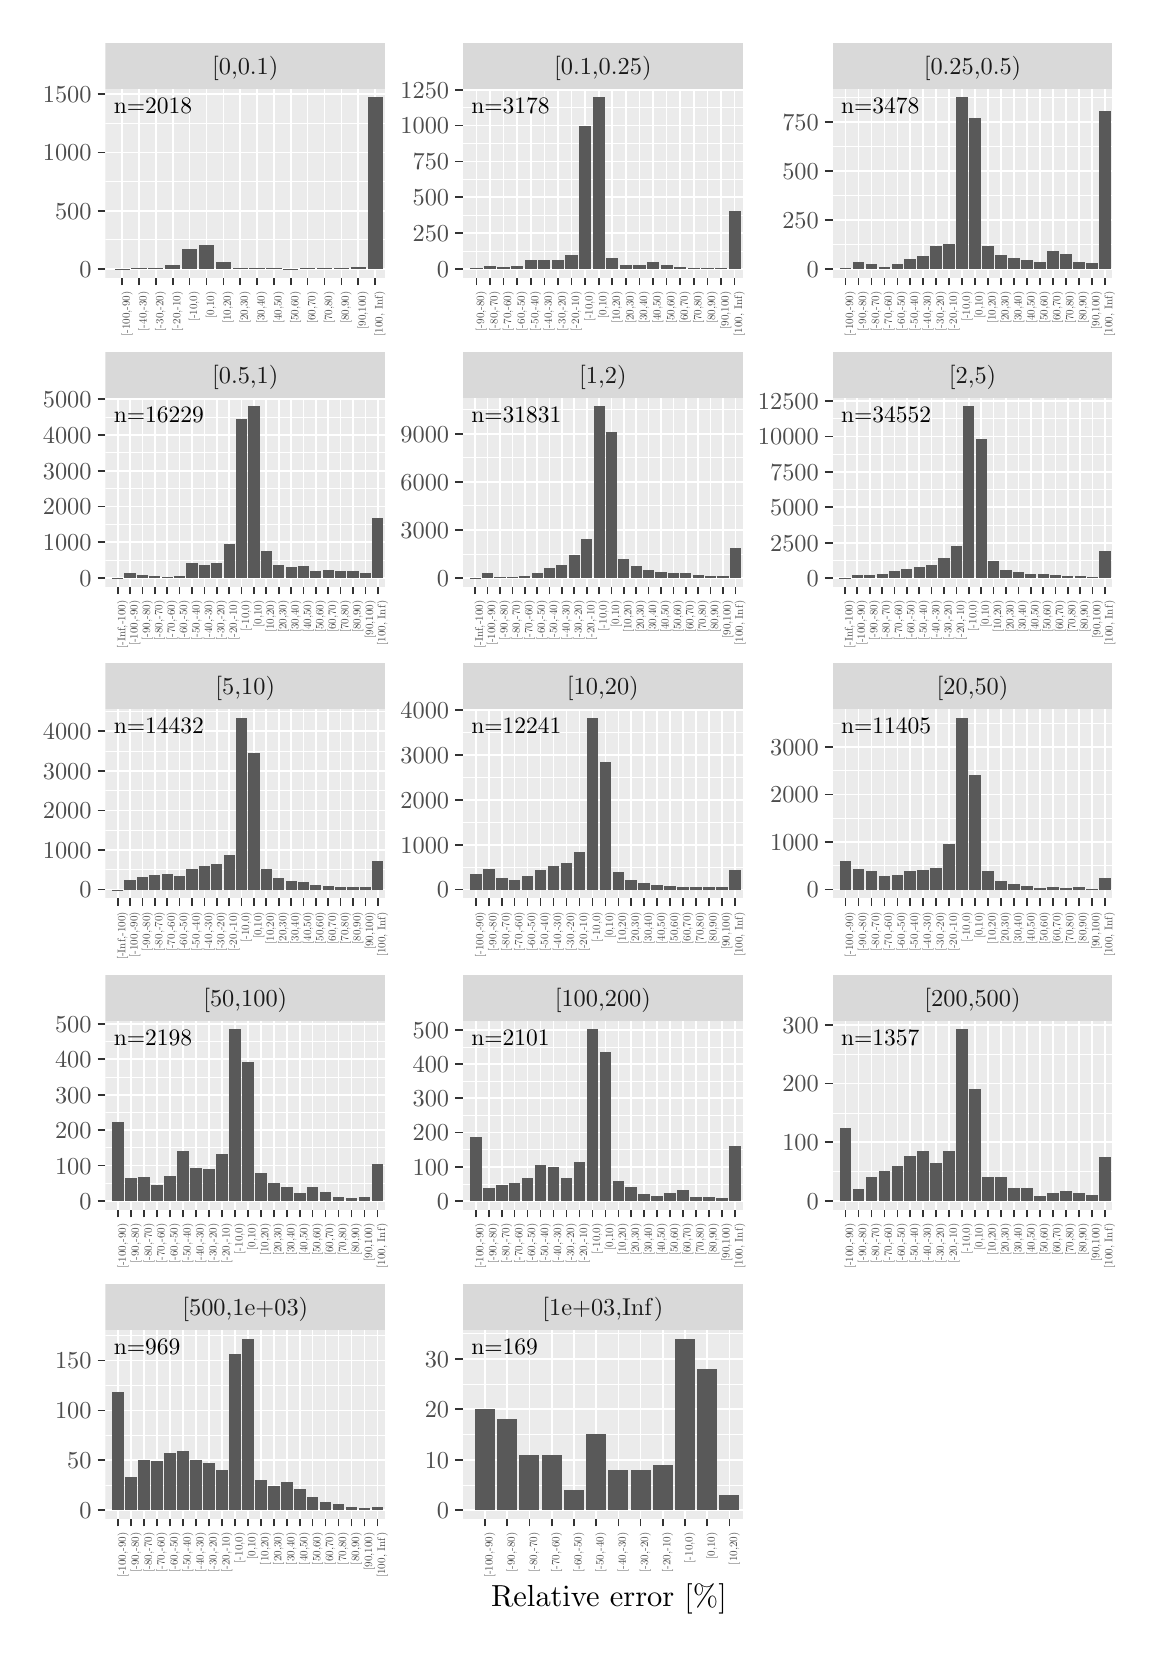
\begin{tikzpicture}[x=1pt,y=1pt]
\definecolor{fillColor}{RGB}{255,255,255}
\path[use as bounding box,fill=fillColor,fill opacity=0.00] (0,0) rectangle (397.48,578.16);
\begin{scope}
\path[clip] (  0.00,  0.00) rectangle (397.48,578.16);
\definecolor{drawColor}{RGB}{255,255,255}
\definecolor{fillColor}{RGB}{255,255,255}

\path[draw=drawColor,line width= 0.6pt,line join=round,line cap=round,fill=fillColor] (  0.00,  0.00) rectangle (397.48,578.16);
\end{scope}
\begin{scope}
\path[clip] ( 28.05,487.87) rectangle (129.20,556.09);
\definecolor{fillColor}{gray}{0.92}

\path[fill=fillColor] ( 28.05,487.87) rectangle (129.20,556.09);
\definecolor{drawColor}{RGB}{255,255,255}

\path[draw=drawColor,line width= 0.3pt,line join=round] ( 28.05,501.49) --
	(129.20,501.49);

\path[draw=drawColor,line width= 0.3pt,line join=round] ( 28.05,522.52) --
	(129.20,522.52);

\path[draw=drawColor,line width= 0.3pt,line join=round] ( 28.05,543.56) --
	(129.20,543.56);

\path[draw=drawColor,line width= 0.6pt,line join=round] ( 28.05,490.97) --
	(129.20,490.97);

\path[draw=drawColor,line width= 0.6pt,line join=round] ( 28.05,512.01) --
	(129.20,512.01);

\path[draw=drawColor,line width= 0.6pt,line join=round] ( 28.05,533.04) --
	(129.20,533.04);

\path[draw=drawColor,line width= 0.6pt,line join=round] ( 28.05,554.08) --
	(129.20,554.08);

\path[draw=drawColor,line width= 0.6pt,line join=round] ( 34.14,487.87) --
	( 34.14,556.09);

\path[draw=drawColor,line width= 0.6pt,line join=round] ( 40.23,487.87) --
	( 40.23,556.09);

\path[draw=drawColor,line width= 0.6pt,line join=round] ( 46.33,487.87) --
	( 46.33,556.09);

\path[draw=drawColor,line width= 0.6pt,line join=round] ( 52.42,487.87) --
	( 52.42,556.09);

\path[draw=drawColor,line width= 0.6pt,line join=round] ( 58.51,487.87) --
	( 58.51,556.09);

\path[draw=drawColor,line width= 0.6pt,line join=round] ( 64.61,487.87) --
	( 64.61,556.09);

\path[draw=drawColor,line width= 0.6pt,line join=round] ( 70.70,487.87) --
	( 70.70,556.09);

\path[draw=drawColor,line width= 0.6pt,line join=round] ( 76.79,487.87) --
	( 76.79,556.09);

\path[draw=drawColor,line width= 0.6pt,line join=round] ( 82.89,487.87) --
	( 82.89,556.09);

\path[draw=drawColor,line width= 0.6pt,line join=round] ( 88.98,487.87) --
	( 88.98,556.09);

\path[draw=drawColor,line width= 0.6pt,line join=round] ( 95.07,487.87) --
	( 95.07,556.09);

\path[draw=drawColor,line width= 0.6pt,line join=round] (101.17,487.87) --
	(101.17,556.09);

\path[draw=drawColor,line width= 0.6pt,line join=round] (107.26,487.87) --
	(107.26,556.09);

\path[draw=drawColor,line width= 0.6pt,line join=round] (113.35,487.87) --
	(113.35,556.09);

\path[draw=drawColor,line width= 0.6pt,line join=round] (119.45,487.87) --
	(119.45,556.09);

\path[draw=drawColor,line width= 0.6pt,line join=round] (125.54,487.87) --
	(125.54,556.09);
\definecolor{fillColor}{gray}{0.35}

\path[fill=fillColor] ( 31.40,490.97) rectangle ( 36.88,491.05);

\path[fill=fillColor] ( 37.49,490.97) rectangle ( 42.97,491.14);

\path[fill=fillColor] ( 43.58,490.97) rectangle ( 49.07,491.22);

\path[fill=fillColor] ( 49.68,490.97) rectangle ( 55.16,492.48);

\path[fill=fillColor] ( 55.77,490.97) rectangle ( 61.25,498.04);

\path[fill=fillColor] ( 61.86,490.97) rectangle ( 67.35,499.76);

\path[fill=fillColor] ( 67.96,490.97) rectangle ( 73.44,493.32);

\path[fill=fillColor] ( 74.05,490.97) rectangle ( 79.53,491.39);

\path[fill=fillColor] ( 80.14,490.97) rectangle ( 85.63,491.26);

\path[fill=fillColor] ( 86.24,490.97) rectangle ( 91.72,491.14);

\path[fill=fillColor] ( 92.33,490.97) rectangle ( 97.81,491.05);

\path[fill=fillColor] ( 98.42,490.97) rectangle (103.91,491.22);

\path[fill=fillColor] (104.52,490.97) rectangle (110.00,491.30);

\path[fill=fillColor] (110.61,490.97) rectangle (116.09,491.43);

\path[fill=fillColor] (116.70,490.97) rectangle (122.19,491.60);

\path[fill=fillColor] (122.80,490.97) rectangle (128.28,552.99);
\definecolor{drawColor}{RGB}{0,0,0}

\node[text=drawColor,anchor=base,inner sep=0pt, outer sep=0pt, scale=  0.85] at ( 45.28,547.20) {n=2018};
\end{scope}
\begin{scope}
\path[clip] ( 28.05,376.18) rectangle (129.20,444.40);
\definecolor{fillColor}{gray}{0.92}

\path[fill=fillColor] ( 28.05,376.18) rectangle (129.20,444.40);
\definecolor{drawColor}{RGB}{255,255,255}

\path[draw=drawColor,line width= 0.3pt,line join=round] ( 28.05,385.75) --
	(129.20,385.75);

\path[draw=drawColor,line width= 0.3pt,line join=round] ( 28.05,398.67) --
	(129.20,398.67);

\path[draw=drawColor,line width= 0.3pt,line join=round] ( 28.05,411.60) --
	(129.20,411.60);

\path[draw=drawColor,line width= 0.3pt,line join=round] ( 28.05,424.53) --
	(129.20,424.53);

\path[draw=drawColor,line width= 0.3pt,line join=round] ( 28.05,437.45) --
	(129.20,437.45);

\path[draw=drawColor,line width= 0.6pt,line join=round] ( 28.05,379.28) --
	(129.20,379.28);

\path[draw=drawColor,line width= 0.6pt,line join=round] ( 28.05,392.21) --
	(129.20,392.21);

\path[draw=drawColor,line width= 0.6pt,line join=round] ( 28.05,405.14) --
	(129.20,405.14);

\path[draw=drawColor,line width= 0.6pt,line join=round] ( 28.05,418.06) --
	(129.20,418.06);

\path[draw=drawColor,line width= 0.6pt,line join=round] ( 28.05,430.99) --
	(129.20,430.99);

\path[draw=drawColor,line width= 0.6pt,line join=round] ( 28.05,443.91) --
	(129.20,443.91);

\path[draw=drawColor,line width= 0.6pt,line join=round] ( 32.52,376.18) --
	( 32.52,444.40);

\path[draw=drawColor,line width= 0.6pt,line join=round] ( 37.00,376.18) --
	( 37.00,444.40);

\path[draw=drawColor,line width= 0.6pt,line join=round] ( 41.47,376.18) --
	( 41.47,444.40);

\path[draw=drawColor,line width= 0.6pt,line join=round] ( 45.95,376.18) --
	( 45.95,444.40);

\path[draw=drawColor,line width= 0.6pt,line join=round] ( 50.42,376.18) --
	( 50.42,444.40);

\path[draw=drawColor,line width= 0.6pt,line join=round] ( 54.90,376.18) --
	( 54.90,444.40);

\path[draw=drawColor,line width= 0.6pt,line join=round] ( 59.38,376.18) --
	( 59.38,444.40);

\path[draw=drawColor,line width= 0.6pt,line join=round] ( 63.85,376.18) --
	( 63.85,444.40);

\path[draw=drawColor,line width= 0.6pt,line join=round] ( 68.33,376.18) --
	( 68.33,444.40);

\path[draw=drawColor,line width= 0.6pt,line join=round] ( 72.80,376.18) --
	( 72.80,444.40);

\path[draw=drawColor,line width= 0.6pt,line join=round] ( 77.28,376.18) --
	( 77.28,444.40);

\path[draw=drawColor,line width= 0.6pt,line join=round] ( 81.75,376.18) --
	( 81.75,444.40);

\path[draw=drawColor,line width= 0.6pt,line join=round] ( 86.23,376.18) --
	( 86.23,444.40);

\path[draw=drawColor,line width= 0.6pt,line join=round] ( 90.70,376.18) --
	( 90.70,444.40);

\path[draw=drawColor,line width= 0.6pt,line join=round] ( 95.18,376.18) --
	( 95.18,444.40);

\path[draw=drawColor,line width= 0.6pt,line join=round] ( 99.66,376.18) --
	( 99.66,444.40);

\path[draw=drawColor,line width= 0.6pt,line join=round] (104.13,376.18) --
	(104.13,444.40);

\path[draw=drawColor,line width= 0.6pt,line join=round] (108.61,376.18) --
	(108.61,444.40);

\path[draw=drawColor,line width= 0.6pt,line join=round] (113.08,376.18) --
	(113.08,444.40);

\path[draw=drawColor,line width= 0.6pt,line join=round] (117.56,376.18) --
	(117.56,444.40);

\path[draw=drawColor,line width= 0.6pt,line join=round] (122.03,376.18) --
	(122.03,444.40);

\path[draw=drawColor,line width= 0.6pt,line join=round] (126.51,376.18) --
	(126.51,444.40);
\definecolor{fillColor}{gray}{0.35}

\path[fill=fillColor] ( 30.51,379.28) rectangle ( 34.54,379.30);

\path[fill=fillColor] ( 34.98,379.28) rectangle ( 39.01,381.09);

\path[fill=fillColor] ( 39.46,379.28) rectangle ( 43.49,380.45);

\path[fill=fillColor] ( 43.93,379.28) rectangle ( 47.96,379.87);

\path[fill=fillColor] ( 48.41,379.28) rectangle ( 52.44,379.81);

\path[fill=fillColor] ( 52.89,379.28) rectangle ( 56.91,380.10);

\path[fill=fillColor] ( 57.36,379.28) rectangle ( 61.39,384.80);

\path[fill=fillColor] ( 61.84,379.28) rectangle ( 65.86,383.90);

\path[fill=fillColor] ( 66.31,379.28) rectangle ( 70.34,384.87);

\path[fill=fillColor] ( 70.79,379.28) rectangle ( 74.82,391.71);

\path[fill=fillColor] ( 75.26,379.28) rectangle ( 79.29,436.72);

\path[fill=fillColor] ( 79.74,379.28) rectangle ( 83.77,441.30);

\path[fill=fillColor] ( 84.22,379.28) rectangle ( 88.24,389.21);

\path[fill=fillColor] ( 88.69,379.28) rectangle ( 92.72,384.14);

\path[fill=fillColor] ( 93.17,379.28) rectangle ( 97.19,383.34);

\path[fill=fillColor] ( 97.64,379.28) rectangle (101.67,383.64);

\path[fill=fillColor] (102.12,379.28) rectangle (106.15,381.93);

\path[fill=fillColor] (106.59,379.28) rectangle (110.62,382.28);

\path[fill=fillColor] (111.07,379.28) rectangle (115.10,381.80);

\path[fill=fillColor] (115.54,379.28) rectangle (119.57,381.73);

\path[fill=fillColor] (120.02,379.28) rectangle (124.05,380.96);

\path[fill=fillColor] (124.50,379.28) rectangle (128.52,401.06);
\definecolor{drawColor}{RGB}{0,0,0}

\node[text=drawColor,anchor=base,inner sep=0pt, outer sep=0pt, scale=  0.85] at ( 47.41,435.51) {n=16229};
\end{scope}
\begin{scope}
\path[clip] ( 28.05,263.61) rectangle (129.20,331.83);
\definecolor{fillColor}{gray}{0.92}

\path[fill=fillColor] ( 28.05,263.61) rectangle (129.20,331.83);
\definecolor{drawColor}{RGB}{255,255,255}

\path[draw=drawColor,line width= 0.3pt,line join=round] ( 28.05,273.86) --
	(129.20,273.86);

\path[draw=drawColor,line width= 0.3pt,line join=round] ( 28.05,288.17) --
	(129.20,288.17);

\path[draw=drawColor,line width= 0.3pt,line join=round] ( 28.05,302.47) --
	(129.20,302.47);

\path[draw=drawColor,line width= 0.3pt,line join=round] ( 28.05,316.77) --
	(129.20,316.77);

\path[draw=drawColor,line width= 0.3pt,line join=round] ( 28.05,331.08) --
	(129.20,331.08);

\path[draw=drawColor,line width= 0.6pt,line join=round] ( 28.05,266.71) --
	(129.20,266.71);

\path[draw=drawColor,line width= 0.6pt,line join=round] ( 28.05,281.02) --
	(129.20,281.02);

\path[draw=drawColor,line width= 0.6pt,line join=round] ( 28.05,295.32) --
	(129.20,295.32);

\path[draw=drawColor,line width= 0.6pt,line join=round] ( 28.05,309.62) --
	(129.20,309.62);

\path[draw=drawColor,line width= 0.6pt,line join=round] ( 28.05,323.93) --
	(129.20,323.93);

\path[draw=drawColor,line width= 0.6pt,line join=round] ( 32.52,263.61) --
	( 32.52,331.83);

\path[draw=drawColor,line width= 0.6pt,line join=round] ( 37.00,263.61) --
	( 37.00,331.83);

\path[draw=drawColor,line width= 0.6pt,line join=round] ( 41.47,263.61) --
	( 41.47,331.83);

\path[draw=drawColor,line width= 0.6pt,line join=round] ( 45.95,263.61) --
	( 45.95,331.83);

\path[draw=drawColor,line width= 0.6pt,line join=round] ( 50.42,263.61) --
	( 50.42,331.83);

\path[draw=drawColor,line width= 0.6pt,line join=round] ( 54.90,263.61) --
	( 54.90,331.83);

\path[draw=drawColor,line width= 0.6pt,line join=round] ( 59.38,263.61) --
	( 59.38,331.83);

\path[draw=drawColor,line width= 0.6pt,line join=round] ( 63.85,263.61) --
	( 63.85,331.83);

\path[draw=drawColor,line width= 0.6pt,line join=round] ( 68.33,263.61) --
	( 68.33,331.83);

\path[draw=drawColor,line width= 0.6pt,line join=round] ( 72.80,263.61) --
	( 72.80,331.83);

\path[draw=drawColor,line width= 0.6pt,line join=round] ( 77.28,263.61) --
	( 77.28,331.83);

\path[draw=drawColor,line width= 0.6pt,line join=round] ( 81.75,263.61) --
	( 81.75,331.83);

\path[draw=drawColor,line width= 0.6pt,line join=round] ( 86.23,263.61) --
	( 86.23,331.83);

\path[draw=drawColor,line width= 0.6pt,line join=round] ( 90.70,263.61) --
	( 90.70,331.83);

\path[draw=drawColor,line width= 0.6pt,line join=round] ( 95.18,263.61) --
	( 95.18,331.83);

\path[draw=drawColor,line width= 0.6pt,line join=round] ( 99.66,263.61) --
	( 99.66,331.83);

\path[draw=drawColor,line width= 0.6pt,line join=round] (104.13,263.61) --
	(104.13,331.83);

\path[draw=drawColor,line width= 0.6pt,line join=round] (108.61,263.61) --
	(108.61,331.83);

\path[draw=drawColor,line width= 0.6pt,line join=round] (113.08,263.61) --
	(113.08,331.83);

\path[draw=drawColor,line width= 0.6pt,line join=round] (117.56,263.61) --
	(117.56,331.83);

\path[draw=drawColor,line width= 0.6pt,line join=round] (122.03,263.61) --
	(122.03,331.83);

\path[draw=drawColor,line width= 0.6pt,line join=round] (126.51,263.61) --
	(126.51,331.83);
\definecolor{fillColor}{gray}{0.35}

\path[fill=fillColor] ( 30.51,266.71) rectangle ( 34.54,266.73);

\path[fill=fillColor] ( 34.98,266.71) rectangle ( 39.01,270.24);

\path[fill=fillColor] ( 39.46,266.71) rectangle ( 43.49,271.23);

\path[fill=fillColor] ( 43.93,266.71) rectangle ( 47.96,271.85);

\path[fill=fillColor] ( 48.41,266.71) rectangle ( 52.44,272.18);

\path[fill=fillColor] ( 52.89,266.71) rectangle ( 56.91,271.55);

\path[fill=fillColor] ( 57.36,266.71) rectangle ( 61.39,274.09);

\path[fill=fillColor] ( 61.84,266.71) rectangle ( 65.86,275.38);

\path[fill=fillColor] ( 66.31,266.71) rectangle ( 70.34,276.11);

\path[fill=fillColor] ( 70.79,266.71) rectangle ( 74.82,279.21);

\path[fill=fillColor] ( 75.26,266.71) rectangle ( 79.29,328.73);

\path[fill=fillColor] ( 79.74,266.71) rectangle ( 83.77,316.19);

\path[fill=fillColor] ( 84.22,266.71) rectangle ( 88.24,274.01);

\path[fill=fillColor] ( 88.69,266.71) rectangle ( 92.72,271.07);

\path[fill=fillColor] ( 93.17,266.71) rectangle ( 97.19,269.93);

\path[fill=fillColor] ( 97.64,266.71) rectangle (101.67,269.47);

\path[fill=fillColor] (102.12,266.71) rectangle (106.15,268.21);

\path[fill=fillColor] (106.59,266.71) rectangle (110.62,268.00);

\path[fill=fillColor] (111.07,266.71) rectangle (115.10,267.61);

\path[fill=fillColor] (115.54,266.71) rectangle (119.57,267.50);

\path[fill=fillColor] (120.02,266.71) rectangle (124.05,267.60);

\path[fill=fillColor] (124.50,266.71) rectangle (128.52,277.20);
\definecolor{drawColor}{RGB}{0,0,0}

\node[text=drawColor,anchor=base,inner sep=0pt, outer sep=0pt, scale=  0.85] at ( 47.41,322.94) {n=14432};
\end{scope}
\begin{scope}
\path[clip] ( 28.05,151.04) rectangle (129.20,219.26);
\definecolor{fillColor}{gray}{0.92}

\path[fill=fillColor] ( 28.05,151.04) rectangle (129.20,219.26);
\definecolor{drawColor}{RGB}{255,255,255}

\path[draw=drawColor,line width= 0.3pt,line join=round] ( 28.05,160.55) --
	(129.20,160.55);

\path[draw=drawColor,line width= 0.3pt,line join=round] ( 28.05,173.36) --
	(129.20,173.36);

\path[draw=drawColor,line width= 0.3pt,line join=round] ( 28.05,186.17) --
	(129.20,186.17);

\path[draw=drawColor,line width= 0.3pt,line join=round] ( 28.05,198.99) --
	(129.20,198.99);

\path[draw=drawColor,line width= 0.3pt,line join=round] ( 28.05,211.80) --
	(129.20,211.80);

\path[draw=drawColor,line width= 0.6pt,line join=round] ( 28.05,154.14) --
	(129.20,154.14);

\path[draw=drawColor,line width= 0.6pt,line join=round] ( 28.05,166.95) --
	(129.20,166.95);

\path[draw=drawColor,line width= 0.6pt,line join=round] ( 28.05,179.77) --
	(129.20,179.77);

\path[draw=drawColor,line width= 0.6pt,line join=round] ( 28.05,192.58) --
	(129.20,192.58);

\path[draw=drawColor,line width= 0.6pt,line join=round] ( 28.05,205.40) --
	(129.20,205.40);

\path[draw=drawColor,line width= 0.6pt,line join=round] ( 28.05,218.21) --
	(129.20,218.21);

\path[draw=drawColor,line width= 0.6pt,line join=round] ( 32.73,151.04) --
	( 32.73,219.26);

\path[draw=drawColor,line width= 0.6pt,line join=round] ( 37.41,151.04) --
	( 37.41,219.26);

\path[draw=drawColor,line width= 0.6pt,line join=round] ( 42.09,151.04) --
	( 42.09,219.26);

\path[draw=drawColor,line width= 0.6pt,line join=round] ( 46.78,151.04) --
	( 46.78,219.26);

\path[draw=drawColor,line width= 0.6pt,line join=round] ( 51.46,151.04) --
	( 51.46,219.26);

\path[draw=drawColor,line width= 0.6pt,line join=round] ( 56.14,151.04) --
	( 56.14,219.26);

\path[draw=drawColor,line width= 0.6pt,line join=round] ( 60.83,151.04) --
	( 60.83,219.26);

\path[draw=drawColor,line width= 0.6pt,line join=round] ( 65.51,151.04) --
	( 65.51,219.26);

\path[draw=drawColor,line width= 0.6pt,line join=round] ( 70.19,151.04) --
	( 70.19,219.26);

\path[draw=drawColor,line width= 0.6pt,line join=round] ( 74.87,151.04) --
	( 74.87,219.26);

\path[draw=drawColor,line width= 0.6pt,line join=round] ( 79.56,151.04) --
	( 79.56,219.26);

\path[draw=drawColor,line width= 0.6pt,line join=round] ( 84.24,151.04) --
	( 84.24,219.26);

\path[draw=drawColor,line width= 0.6pt,line join=round] ( 88.92,151.04) --
	( 88.92,219.26);

\path[draw=drawColor,line width= 0.6pt,line join=round] ( 93.61,151.04) --
	( 93.61,219.26);

\path[draw=drawColor,line width= 0.6pt,line join=round] ( 98.29,151.04) --
	( 98.29,219.26);

\path[draw=drawColor,line width= 0.6pt,line join=round] (102.97,151.04) --
	(102.97,219.26);

\path[draw=drawColor,line width= 0.6pt,line join=round] (107.65,151.04) --
	(107.65,219.26);

\path[draw=drawColor,line width= 0.6pt,line join=round] (112.34,151.04) --
	(112.34,219.26);

\path[draw=drawColor,line width= 0.6pt,line join=round] (117.02,151.04) --
	(117.02,219.26);

\path[draw=drawColor,line width= 0.6pt,line join=round] (121.70,151.04) --
	(121.70,219.26);

\path[draw=drawColor,line width= 0.6pt,line join=round] (126.39,151.04) --
	(126.39,219.26);
\definecolor{fillColor}{gray}{0.35}

\path[fill=fillColor] ( 30.62,154.14) rectangle ( 34.84,182.59);

\path[fill=fillColor] ( 35.30,154.14) rectangle ( 39.52,162.60);

\path[fill=fillColor] ( 39.99,154.14) rectangle ( 44.20,162.85);

\path[fill=fillColor] ( 44.67,154.14) rectangle ( 48.88,159.78);

\path[fill=fillColor] ( 49.35,154.14) rectangle ( 53.57,163.11);

\path[fill=fillColor] ( 54.04,154.14) rectangle ( 58.25,172.34);

\path[fill=fillColor] ( 58.72,154.14) rectangle ( 62.93,165.93);

\path[fill=fillColor] ( 63.40,154.14) rectangle ( 67.62,165.67);

\path[fill=fillColor] ( 68.08,154.14) rectangle ( 72.30,171.31);

\path[fill=fillColor] ( 72.77,154.14) rectangle ( 76.98,216.16);

\path[fill=fillColor] ( 77.45,154.14) rectangle ( 81.66,204.24);

\path[fill=fillColor] ( 82.13,154.14) rectangle ( 86.35,164.39);

\path[fill=fillColor] ( 86.82,154.14) rectangle ( 91.03,160.67);

\path[fill=fillColor] ( 91.50,154.14) rectangle ( 95.71,159.14);

\path[fill=fillColor] ( 96.18,154.14) rectangle (100.40,157.09);

\path[fill=fillColor] (100.86,154.14) rectangle (105.08,159.26);

\path[fill=fillColor] (105.55,154.14) rectangle (109.76,157.34);

\path[fill=fillColor] (110.23,154.14) rectangle (114.44,155.68);

\path[fill=fillColor] (114.91,154.14) rectangle (119.13,155.42);

\path[fill=fillColor] (119.60,154.14) rectangle (123.81,155.55);

\path[fill=fillColor] (124.28,154.14) rectangle (128.49,167.47);
\definecolor{drawColor}{RGB}{0,0,0}

\node[text=drawColor,anchor=base,inner sep=0pt, outer sep=0pt, scale=  0.85] at ( 45.28,210.37) {n=2198};
\end{scope}
\begin{scope}
\path[clip] ( 28.05, 39.35) rectangle (129.20,107.58);
\definecolor{fillColor}{gray}{0.92}

\path[fill=fillColor] ( 28.05, 39.35) rectangle (129.20,107.58);
\definecolor{drawColor}{RGB}{255,255,255}

\path[draw=drawColor,line width= 0.3pt,line join=round] ( 28.05, 51.47) --
	(129.20, 51.47);

\path[draw=drawColor,line width= 0.3pt,line join=round] ( 28.05, 69.50) --
	(129.20, 69.50);

\path[draw=drawColor,line width= 0.3pt,line join=round] ( 28.05, 87.53) --
	(129.20, 87.53);

\path[draw=drawColor,line width= 0.3pt,line join=round] ( 28.05,105.56) --
	(129.20,105.56);

\path[draw=drawColor,line width= 0.6pt,line join=round] ( 28.05, 42.46) --
	(129.20, 42.46);

\path[draw=drawColor,line width= 0.6pt,line join=round] ( 28.05, 60.48) --
	(129.20, 60.48);

\path[draw=drawColor,line width= 0.6pt,line join=round] ( 28.05, 78.51) --
	(129.20, 78.51);

\path[draw=drawColor,line width= 0.6pt,line join=round] ( 28.05, 96.54) --
	(129.20, 96.54);

\path[draw=drawColor,line width= 0.6pt,line join=round] ( 32.73, 39.35) --
	( 32.73,107.58);

\path[draw=drawColor,line width= 0.6pt,line join=round] ( 37.41, 39.35) --
	( 37.41,107.58);

\path[draw=drawColor,line width= 0.6pt,line join=round] ( 42.09, 39.35) --
	( 42.09,107.58);

\path[draw=drawColor,line width= 0.6pt,line join=round] ( 46.78, 39.35) --
	( 46.78,107.58);

\path[draw=drawColor,line width= 0.6pt,line join=round] ( 51.46, 39.35) --
	( 51.46,107.58);

\path[draw=drawColor,line width= 0.6pt,line join=round] ( 56.14, 39.35) --
	( 56.14,107.58);

\path[draw=drawColor,line width= 0.6pt,line join=round] ( 60.83, 39.35) --
	( 60.83,107.58);

\path[draw=drawColor,line width= 0.6pt,line join=round] ( 65.51, 39.35) --
	( 65.51,107.58);

\path[draw=drawColor,line width= 0.6pt,line join=round] ( 70.19, 39.35) --
	( 70.19,107.58);

\path[draw=drawColor,line width= 0.6pt,line join=round] ( 74.87, 39.35) --
	( 74.87,107.58);

\path[draw=drawColor,line width= 0.6pt,line join=round] ( 79.56, 39.35) --
	( 79.56,107.58);

\path[draw=drawColor,line width= 0.6pt,line join=round] ( 84.24, 39.35) --
	( 84.24,107.58);

\path[draw=drawColor,line width= 0.6pt,line join=round] ( 88.92, 39.35) --
	( 88.92,107.58);

\path[draw=drawColor,line width= 0.6pt,line join=round] ( 93.61, 39.35) --
	( 93.61,107.58);

\path[draw=drawColor,line width= 0.6pt,line join=round] ( 98.29, 39.35) --
	( 98.29,107.58);

\path[draw=drawColor,line width= 0.6pt,line join=round] (102.97, 39.35) --
	(102.97,107.58);

\path[draw=drawColor,line width= 0.6pt,line join=round] (107.65, 39.35) --
	(107.65,107.58);

\path[draw=drawColor,line width= 0.6pt,line join=round] (112.34, 39.35) --
	(112.34,107.58);

\path[draw=drawColor,line width= 0.6pt,line join=round] (117.02, 39.35) --
	(117.02,107.58);

\path[draw=drawColor,line width= 0.6pt,line join=round] (121.70, 39.35) --
	(121.70,107.58);

\path[draw=drawColor,line width= 0.6pt,line join=round] (126.39, 39.35) --
	(126.39,107.58);
\definecolor{fillColor}{gray}{0.35}

\path[fill=fillColor] ( 30.62, 42.46) rectangle ( 34.84, 85.00);

\path[fill=fillColor] ( 35.30, 42.46) rectangle ( 39.52, 54.35);

\path[fill=fillColor] ( 39.99, 42.46) rectangle ( 44.20, 60.48);

\path[fill=fillColor] ( 44.67, 42.46) rectangle ( 48.88, 60.12);

\path[fill=fillColor] ( 49.35, 42.46) rectangle ( 53.57, 63.01);

\path[fill=fillColor] ( 54.04, 42.46) rectangle ( 58.25, 63.73);

\path[fill=fillColor] ( 58.72, 42.46) rectangle ( 62.93, 60.48);

\path[fill=fillColor] ( 63.40, 42.46) rectangle ( 67.62, 59.40);

\path[fill=fillColor] ( 68.08, 42.46) rectangle ( 72.30, 56.88);

\path[fill=fillColor] ( 72.77, 42.46) rectangle ( 76.98, 98.71);

\path[fill=fillColor] ( 77.45, 42.46) rectangle ( 81.66,104.48);

\path[fill=fillColor] ( 82.13, 42.46) rectangle ( 86.35, 53.27);

\path[fill=fillColor] ( 86.82, 42.46) rectangle ( 91.03, 51.11);

\path[fill=fillColor] ( 91.50, 42.46) rectangle ( 95.71, 52.55);

\path[fill=fillColor] ( 96.18, 42.46) rectangle (100.40, 50.03);

\path[fill=fillColor] (100.86, 42.46) rectangle (105.08, 47.14);

\path[fill=fillColor] (105.55, 42.46) rectangle (109.76, 45.34);

\path[fill=fillColor] (110.23, 42.46) rectangle (114.44, 44.62);

\path[fill=fillColor] (114.91, 42.46) rectangle (119.13, 43.54);

\path[fill=fillColor] (119.60, 42.46) rectangle (123.81, 43.18);

\path[fill=fillColor] (124.28, 42.46) rectangle (128.49, 43.54);
\definecolor{drawColor}{RGB}{0,0,0}

\node[text=drawColor,anchor=base,inner sep=0pt, outer sep=0pt, scale=  0.85] at ( 43.15, 98.69) {n=969};
\end{scope}
\begin{scope}
\path[clip] (157.24,487.87) rectangle (258.39,556.09);
\definecolor{fillColor}{gray}{0.92}

\path[fill=fillColor] (157.24,487.87) rectangle (258.39,556.09);
\definecolor{drawColor}{RGB}{255,255,255}

\path[draw=drawColor,line width= 0.3pt,line join=round] (157.24,497.44) --
	(258.39,497.44);

\path[draw=drawColor,line width= 0.3pt,line join=round] (157.24,510.40) --
	(258.39,510.40);

\path[draw=drawColor,line width= 0.3pt,line join=round] (157.24,523.35) --
	(258.39,523.35);

\path[draw=drawColor,line width= 0.3pt,line join=round] (157.24,536.30) --
	(258.39,536.30);

\path[draw=drawColor,line width= 0.3pt,line join=round] (157.24,549.26) --
	(258.39,549.26);

\path[draw=drawColor,line width= 0.6pt,line join=round] (157.24,490.97) --
	(258.39,490.97);

\path[draw=drawColor,line width= 0.6pt,line join=round] (157.24,503.92) --
	(258.39,503.92);

\path[draw=drawColor,line width= 0.6pt,line join=round] (157.24,516.87) --
	(258.39,516.87);

\path[draw=drawColor,line width= 0.6pt,line join=round] (157.24,529.83) --
	(258.39,529.83);

\path[draw=drawColor,line width= 0.6pt,line join=round] (157.24,542.78) --
	(258.39,542.78);

\path[draw=drawColor,line width= 0.6pt,line join=round] (157.24,555.73) --
	(258.39,555.73);

\path[draw=drawColor,line width= 0.6pt,line join=round] (162.15,487.87) --
	(162.15,556.09);

\path[draw=drawColor,line width= 0.6pt,line join=round] (167.06,487.87) --
	(167.06,556.09);

\path[draw=drawColor,line width= 0.6pt,line join=round] (171.97,487.87) --
	(171.97,556.09);

\path[draw=drawColor,line width= 0.6pt,line join=round] (176.88,487.87) --
	(176.88,556.09);

\path[draw=drawColor,line width= 0.6pt,line join=round] (181.79,487.87) --
	(181.79,556.09);

\path[draw=drawColor,line width= 0.6pt,line join=round] (186.70,487.87) --
	(186.70,556.09);

\path[draw=drawColor,line width= 0.6pt,line join=round] (191.61,487.87) --
	(191.61,556.09);

\path[draw=drawColor,line width= 0.6pt,line join=round] (196.52,487.87) --
	(196.52,556.09);

\path[draw=drawColor,line width= 0.6pt,line join=round] (201.43,487.87) --
	(201.43,556.09);

\path[draw=drawColor,line width= 0.6pt,line join=round] (206.34,487.87) --
	(206.34,556.09);

\path[draw=drawColor,line width= 0.6pt,line join=round] (211.25,487.87) --
	(211.25,556.09);

\path[draw=drawColor,line width= 0.6pt,line join=round] (216.16,487.87) --
	(216.16,556.09);

\path[draw=drawColor,line width= 0.6pt,line join=round] (221.07,487.87) --
	(221.07,556.09);

\path[draw=drawColor,line width= 0.6pt,line join=round] (225.98,487.87) --
	(225.98,556.09);

\path[draw=drawColor,line width= 0.6pt,line join=round] (230.89,487.87) --
	(230.89,556.09);

\path[draw=drawColor,line width= 0.6pt,line join=round] (235.80,487.87) --
	(235.80,556.09);

\path[draw=drawColor,line width= 0.6pt,line join=round] (240.71,487.87) --
	(240.71,556.09);

\path[draw=drawColor,line width= 0.6pt,line join=round] (245.62,487.87) --
	(245.62,556.09);

\path[draw=drawColor,line width= 0.6pt,line join=round] (250.53,487.87) --
	(250.53,556.09);

\path[draw=drawColor,line width= 0.6pt,line join=round] (255.44,487.87) --
	(255.44,556.09);
\definecolor{fillColor}{gray}{0.35}

\path[fill=fillColor] (159.94,490.97) rectangle (164.36,491.23);

\path[fill=fillColor] (164.85,490.97) rectangle (169.27,492.11);

\path[fill=fillColor] (169.76,490.97) rectangle (174.18,491.59);

\path[fill=fillColor] (174.67,490.97) rectangle (179.09,492.06);

\path[fill=fillColor] (179.58,490.97) rectangle (184.00,494.13);

\path[fill=fillColor] (184.49,490.97) rectangle (188.91,494.28);

\path[fill=fillColor] (189.40,490.97) rectangle (193.82,494.28);

\path[fill=fillColor] (194.31,490.97) rectangle (198.73,495.84);

\path[fill=fillColor] (199.22,490.97) rectangle (203.64,542.57);

\path[fill=fillColor] (204.13,490.97) rectangle (208.55,552.99);

\path[fill=fillColor] (209.04,490.97) rectangle (213.46,494.75);

\path[fill=fillColor] (213.95,490.97) rectangle (218.37,492.26);

\path[fill=fillColor] (218.86,490.97) rectangle (223.28,492.57);

\path[fill=fillColor] (223.77,490.97) rectangle (228.19,493.40);

\path[fill=fillColor] (228.68,490.97) rectangle (233.10,492.37);

\path[fill=fillColor] (233.59,490.97) rectangle (238.01,491.59);

\path[fill=fillColor] (238.50,490.97) rectangle (242.92,491.38);

\path[fill=fillColor] (243.41,490.97) rectangle (247.83,491.33);

\path[fill=fillColor] (248.32,490.97) rectangle (252.74,491.49);

\path[fill=fillColor] (253.24,490.97) rectangle (257.65,511.80);
\definecolor{drawColor}{RGB}{0,0,0}

\node[text=drawColor,anchor=base,inner sep=0pt, outer sep=0pt, scale=  0.85] at (174.48,547.20) {n=3178};
\end{scope}
\begin{scope}
\path[clip] (157.24,376.18) rectangle (258.39,444.40);
\definecolor{fillColor}{gray}{0.92}

\path[fill=fillColor] (157.24,376.18) rectangle (258.39,444.40);
\definecolor{drawColor}{RGB}{255,255,255}

\path[draw=drawColor,line width= 0.3pt,line join=round] (157.24,387.97) --
	(258.39,387.97);

\path[draw=drawColor,line width= 0.3pt,line join=round] (157.24,405.35) --
	(258.39,405.35);

\path[draw=drawColor,line width= 0.3pt,line join=round] (157.24,422.74) --
	(258.39,422.74);

\path[draw=drawColor,line width= 0.3pt,line join=round] (157.24,440.12) --
	(258.39,440.12);

\path[draw=drawColor,line width= 0.6pt,line join=round] (157.24,379.28) --
	(258.39,379.28);

\path[draw=drawColor,line width= 0.6pt,line join=round] (157.24,396.66) --
	(258.39,396.66);

\path[draw=drawColor,line width= 0.6pt,line join=round] (157.24,414.05) --
	(258.39,414.05);

\path[draw=drawColor,line width= 0.6pt,line join=round] (157.24,431.43) --
	(258.39,431.43);

\path[draw=drawColor,line width= 0.6pt,line join=round] (161.72,376.18) --
	(161.72,444.40);

\path[draw=drawColor,line width= 0.6pt,line join=round] (166.19,376.18) --
	(166.19,444.40);

\path[draw=drawColor,line width= 0.6pt,line join=round] (170.67,376.18) --
	(170.67,444.40);

\path[draw=drawColor,line width= 0.6pt,line join=round] (175.14,376.18) --
	(175.14,444.40);

\path[draw=drawColor,line width= 0.6pt,line join=round] (179.62,376.18) --
	(179.62,444.40);

\path[draw=drawColor,line width= 0.6pt,line join=round] (184.10,376.18) --
	(184.10,444.40);

\path[draw=drawColor,line width= 0.6pt,line join=round] (188.57,376.18) --
	(188.57,444.40);

\path[draw=drawColor,line width= 0.6pt,line join=round] (193.05,376.18) --
	(193.05,444.40);

\path[draw=drawColor,line width= 0.6pt,line join=round] (197.52,376.18) --
	(197.52,444.40);

\path[draw=drawColor,line width= 0.6pt,line join=round] (202.00,376.18) --
	(202.00,444.40);

\path[draw=drawColor,line width= 0.6pt,line join=round] (206.47,376.18) --
	(206.47,444.40);

\path[draw=drawColor,line width= 0.6pt,line join=round] (210.95,376.18) --
	(210.95,444.40);

\path[draw=drawColor,line width= 0.6pt,line join=round] (215.42,376.18) --
	(215.42,444.40);

\path[draw=drawColor,line width= 0.6pt,line join=round] (219.90,376.18) --
	(219.90,444.40);

\path[draw=drawColor,line width= 0.6pt,line join=round] (224.38,376.18) --
	(224.38,444.40);

\path[draw=drawColor,line width= 0.6pt,line join=round] (228.85,376.18) --
	(228.85,444.40);

\path[draw=drawColor,line width= 0.6pt,line join=round] (233.33,376.18) --
	(233.33,444.40);

\path[draw=drawColor,line width= 0.6pt,line join=round] (237.80,376.18) --
	(237.80,444.40);

\path[draw=drawColor,line width= 0.6pt,line join=round] (242.28,376.18) --
	(242.28,444.40);

\path[draw=drawColor,line width= 0.6pt,line join=round] (246.75,376.18) --
	(246.75,444.40);

\path[draw=drawColor,line width= 0.6pt,line join=round] (251.23,376.18) --
	(251.23,444.40);

\path[draw=drawColor,line width= 0.6pt,line join=round] (255.71,376.18) --
	(255.71,444.40);
\definecolor{fillColor}{gray}{0.35}

\path[fill=fillColor] (159.70,379.28) rectangle (163.73,379.30);

\path[fill=fillColor] (164.18,379.28) rectangle (168.21,380.99);

\path[fill=fillColor] (168.65,379.28) rectangle (172.68,379.65);

\path[fill=fillColor] (173.13,379.28) rectangle (177.16,379.75);

\path[fill=fillColor] (177.61,379.28) rectangle (181.63,380.00);

\path[fill=fillColor] (182.08,379.28) rectangle (186.11,381.21);

\path[fill=fillColor] (186.56,379.28) rectangle (190.58,382.96);

\path[fill=fillColor] (191.03,379.28) rectangle (195.06,383.88);

\path[fill=fillColor] (195.51,379.28) rectangle (199.54,387.71);

\path[fill=fillColor] (199.98,379.28) rectangle (204.01,393.36);

\path[fill=fillColor] (204.46,379.28) rectangle (208.49,441.30);

\path[fill=fillColor] (208.93,379.28) rectangle (212.96,431.95);

\path[fill=fillColor] (213.41,379.28) rectangle (217.44,386.29);

\path[fill=fillColor] (217.89,379.28) rectangle (221.91,383.77);

\path[fill=fillColor] (222.36,379.28) rectangle (226.39,382.30);

\path[fill=fillColor] (226.84,379.28) rectangle (230.87,381.45);

\path[fill=fillColor] (231.31,379.28) rectangle (235.34,380.97);

\path[fill=fillColor] (235.79,379.28) rectangle (239.82,380.95);

\path[fill=fillColor] (240.26,379.28) rectangle (244.29,380.42);

\path[fill=fillColor] (244.74,379.28) rectangle (248.77,380.18);

\path[fill=fillColor] (249.22,379.28) rectangle (253.24,380.02);

\path[fill=fillColor] (253.69,379.28) rectangle (257.72,390.25);
\definecolor{drawColor}{RGB}{0,0,0}

\node[text=drawColor,anchor=base,inner sep=0pt, outer sep=0pt, scale=  0.85] at (176.61,435.51) {n=31831};
\end{scope}
\begin{scope}
\path[clip] (157.24,263.61) rectangle (258.39,331.83);
\definecolor{fillColor}{gray}{0.92}

\path[fill=fillColor] (157.24,263.61) rectangle (258.39,331.83);
\definecolor{drawColor}{RGB}{255,255,255}

\path[draw=drawColor,line width= 0.3pt,line join=round] (157.24,274.82) --
	(258.39,274.82);

\path[draw=drawColor,line width= 0.3pt,line join=round] (157.24,291.03) --
	(258.39,291.03);

\path[draw=drawColor,line width= 0.3pt,line join=round] (157.24,307.25) --
	(258.39,307.25);

\path[draw=drawColor,line width= 0.3pt,line join=round] (157.24,323.46) --
	(258.39,323.46);

\path[draw=drawColor,line width= 0.6pt,line join=round] (157.24,266.71) --
	(258.39,266.71);

\path[draw=drawColor,line width= 0.6pt,line join=round] (157.24,282.93) --
	(258.39,282.93);

\path[draw=drawColor,line width= 0.6pt,line join=round] (157.24,299.14) --
	(258.39,299.14);

\path[draw=drawColor,line width= 0.6pt,line join=round] (157.24,315.35) --
	(258.39,315.35);

\path[draw=drawColor,line width= 0.6pt,line join=round] (157.24,331.57) --
	(258.39,331.57);

\path[draw=drawColor,line width= 0.6pt,line join=round] (161.92,263.61) --
	(161.92,331.83);

\path[draw=drawColor,line width= 0.6pt,line join=round] (166.61,263.61) --
	(166.61,331.83);

\path[draw=drawColor,line width= 0.6pt,line join=round] (171.29,263.61) --
	(171.29,331.83);

\path[draw=drawColor,line width= 0.6pt,line join=round] (175.97,263.61) --
	(175.97,331.83);

\path[draw=drawColor,line width= 0.6pt,line join=round] (180.66,263.61) --
	(180.66,331.83);

\path[draw=drawColor,line width= 0.6pt,line join=round] (185.34,263.61) --
	(185.34,331.83);

\path[draw=drawColor,line width= 0.6pt,line join=round] (190.02,263.61) --
	(190.02,331.83);

\path[draw=drawColor,line width= 0.6pt,line join=round] (194.70,263.61) --
	(194.70,331.83);

\path[draw=drawColor,line width= 0.6pt,line join=round] (199.39,263.61) --
	(199.39,331.83);

\path[draw=drawColor,line width= 0.6pt,line join=round] (204.07,263.61) --
	(204.07,331.83);

\path[draw=drawColor,line width= 0.6pt,line join=round] (208.75,263.61) --
	(208.75,331.83);

\path[draw=drawColor,line width= 0.6pt,line join=round] (213.44,263.61) --
	(213.44,331.83);

\path[draw=drawColor,line width= 0.6pt,line join=round] (218.12,263.61) --
	(218.12,331.83);

\path[draw=drawColor,line width= 0.6pt,line join=round] (222.80,263.61) --
	(222.80,331.83);

\path[draw=drawColor,line width= 0.6pt,line join=round] (227.48,263.61) --
	(227.48,331.83);

\path[draw=drawColor,line width= 0.6pt,line join=round] (232.17,263.61) --
	(232.17,331.83);

\path[draw=drawColor,line width= 0.6pt,line join=round] (236.85,263.61) --
	(236.85,331.83);

\path[draw=drawColor,line width= 0.6pt,line join=round] (241.53,263.61) --
	(241.53,331.83);

\path[draw=drawColor,line width= 0.6pt,line join=round] (246.22,263.61) --
	(246.22,331.83);

\path[draw=drawColor,line width= 0.6pt,line join=round] (250.90,263.61) --
	(250.90,331.83);

\path[draw=drawColor,line width= 0.6pt,line join=round] (255.58,263.61) --
	(255.58,331.83);
\definecolor{fillColor}{gray}{0.35}

\path[fill=fillColor] (159.82,266.71) rectangle (164.03,272.47);

\path[fill=fillColor] (164.50,266.71) rectangle (168.71,274.11);

\path[fill=fillColor] (169.18,266.71) rectangle (173.40,270.72);

\path[fill=fillColor] (173.87,266.71) rectangle (178.08,270.20);

\path[fill=fillColor] (178.55,266.71) rectangle (182.76,271.58);

\path[fill=fillColor] (183.23,266.71) rectangle (187.45,273.86);

\path[fill=fillColor] (187.91,266.71) rectangle (192.13,275.31);

\path[fill=fillColor] (192.60,266.71) rectangle (196.81,276.38);

\path[fill=fillColor] (197.28,266.71) rectangle (201.49,280.23);

\path[fill=fillColor] (201.96,266.71) rectangle (206.18,328.73);

\path[fill=fillColor] (206.65,266.71) rectangle (210.86,312.76);

\path[fill=fillColor] (211.33,266.71) rectangle (215.54,272.91);

\path[fill=fillColor] (216.01,266.71) rectangle (220.23,270.23);

\path[fill=fillColor] (220.69,266.71) rectangle (224.91,269.03);

\path[fill=fillColor] (225.38,266.71) rectangle (229.59,268.54);

\path[fill=fillColor] (230.06,266.71) rectangle (234.27,267.86);

\path[fill=fillColor] (234.74,266.71) rectangle (238.96,267.77);

\path[fill=fillColor] (239.43,266.71) rectangle (243.64,267.70);

\path[fill=fillColor] (244.11,266.71) rectangle (248.32,267.47);

\path[fill=fillColor] (248.79,266.71) rectangle (253.01,267.73);

\path[fill=fillColor] (253.47,266.71) rectangle (257.69,273.85);
\definecolor{drawColor}{RGB}{0,0,0}

\node[text=drawColor,anchor=base,inner sep=0pt, outer sep=0pt, scale=  0.85] at (176.61,322.94) {n=12241};
\end{scope}
\begin{scope}
\path[clip] (157.24,151.04) rectangle (258.39,219.26);
\definecolor{fillColor}{gray}{0.92}

\path[fill=fillColor] (157.24,151.04) rectangle (258.39,219.26);
\definecolor{drawColor}{RGB}{255,255,255}

\path[draw=drawColor,line width= 0.3pt,line join=round] (157.24,160.33) --
	(258.39,160.33);

\path[draw=drawColor,line width= 0.3pt,line join=round] (157.24,172.71) --
	(258.39,172.71);

\path[draw=drawColor,line width= 0.3pt,line join=round] (157.24,185.09) --
	(258.39,185.09);

\path[draw=drawColor,line width= 0.3pt,line join=round] (157.24,197.47) --
	(258.39,197.47);

\path[draw=drawColor,line width= 0.3pt,line join=round] (157.24,209.85) --
	(258.39,209.85);

\path[draw=drawColor,line width= 0.6pt,line join=round] (157.24,154.14) --
	(258.39,154.14);

\path[draw=drawColor,line width= 0.6pt,line join=round] (157.24,166.52) --
	(258.39,166.52);

\path[draw=drawColor,line width= 0.6pt,line join=round] (157.24,178.90) --
	(258.39,178.90);

\path[draw=drawColor,line width= 0.6pt,line join=round] (157.24,191.28) --
	(258.39,191.28);

\path[draw=drawColor,line width= 0.6pt,line join=round] (157.24,203.66) --
	(258.39,203.66);

\path[draw=drawColor,line width= 0.6pt,line join=round] (157.24,216.04) --
	(258.39,216.04);

\path[draw=drawColor,line width= 0.6pt,line join=round] (161.92,151.04) --
	(161.92,219.26);

\path[draw=drawColor,line width= 0.6pt,line join=round] (166.61,151.04) --
	(166.61,219.26);

\path[draw=drawColor,line width= 0.6pt,line join=round] (171.29,151.04) --
	(171.29,219.26);

\path[draw=drawColor,line width= 0.6pt,line join=round] (175.97,151.04) --
	(175.97,219.26);

\path[draw=drawColor,line width= 0.6pt,line join=round] (180.66,151.04) --
	(180.66,219.26);

\path[draw=drawColor,line width= 0.6pt,line join=round] (185.34,151.04) --
	(185.34,219.26);

\path[draw=drawColor,line width= 0.6pt,line join=round] (190.02,151.04) --
	(190.02,219.26);

\path[draw=drawColor,line width= 0.6pt,line join=round] (194.70,151.04) --
	(194.70,219.26);

\path[draw=drawColor,line width= 0.6pt,line join=round] (199.39,151.04) --
	(199.39,219.26);

\path[draw=drawColor,line width= 0.6pt,line join=round] (204.07,151.04) --
	(204.07,219.26);

\path[draw=drawColor,line width= 0.6pt,line join=round] (208.75,151.04) --
	(208.75,219.26);

\path[draw=drawColor,line width= 0.6pt,line join=round] (213.44,151.04) --
	(213.44,219.26);

\path[draw=drawColor,line width= 0.6pt,line join=round] (218.12,151.04) --
	(218.12,219.26);

\path[draw=drawColor,line width= 0.6pt,line join=round] (222.80,151.04) --
	(222.80,219.26);

\path[draw=drawColor,line width= 0.6pt,line join=round] (227.48,151.04) --
	(227.48,219.26);

\path[draw=drawColor,line width= 0.6pt,line join=round] (232.17,151.04) --
	(232.17,219.26);

\path[draw=drawColor,line width= 0.6pt,line join=round] (236.85,151.04) --
	(236.85,219.26);

\path[draw=drawColor,line width= 0.6pt,line join=round] (241.53,151.04) --
	(241.53,219.26);

\path[draw=drawColor,line width= 0.6pt,line join=round] (246.22,151.04) --
	(246.22,219.26);

\path[draw=drawColor,line width= 0.6pt,line join=round] (250.90,151.04) --
	(250.90,219.26);

\path[draw=drawColor,line width= 0.6pt,line join=round] (255.58,151.04) --
	(255.58,219.26);
\definecolor{fillColor}{gray}{0.35}

\path[fill=fillColor] (159.82,154.14) rectangle (164.03,177.41);

\path[fill=fillColor] (164.50,154.14) rectangle (168.71,158.84);

\path[fill=fillColor] (169.18,154.14) rectangle (173.40,160.08);

\path[fill=fillColor] (173.87,154.14) rectangle (178.08,160.58);

\path[fill=fillColor] (178.55,154.14) rectangle (182.76,162.56);

\path[fill=fillColor] (183.23,154.14) rectangle (187.45,167.26);

\path[fill=fillColor] (187.91,154.14) rectangle (192.13,166.52);

\path[fill=fillColor] (192.60,154.14) rectangle (196.81,162.43);

\path[fill=fillColor] (197.28,154.14) rectangle (201.49,168.38);

\path[fill=fillColor] (201.96,154.14) rectangle (206.18,216.16);

\path[fill=fillColor] (206.65,154.14) rectangle (210.86,207.99);

\path[fill=fillColor] (211.33,154.14) rectangle (215.54,161.32);

\path[fill=fillColor] (216.01,154.14) rectangle (220.23,159.21);

\path[fill=fillColor] (220.69,154.14) rectangle (224.91,156.86);

\path[fill=fillColor] (225.38,154.14) rectangle (229.59,156.00);

\path[fill=fillColor] (230.06,154.14) rectangle (234.27,157.11);

\path[fill=fillColor] (234.74,154.14) rectangle (238.96,158.10);

\path[fill=fillColor] (239.43,154.14) rectangle (243.64,155.62);

\path[fill=fillColor] (244.11,154.14) rectangle (248.32,155.50);

\path[fill=fillColor] (248.79,154.14) rectangle (253.01,155.13);

\path[fill=fillColor] (253.47,154.14) rectangle (257.69,173.95);
\definecolor{drawColor}{RGB}{0,0,0}

\node[text=drawColor,anchor=base,inner sep=0pt, outer sep=0pt, scale=  0.85] at (174.48,210.37) {n=2101};
\end{scope}
\begin{scope}
\path[clip] (157.24, 39.35) rectangle (258.39,107.58);
\definecolor{fillColor}{gray}{0.92}

\path[fill=fillColor] (157.24, 39.35) rectangle (258.39,107.58);
\definecolor{drawColor}{RGB}{255,255,255}

\path[draw=drawColor,line width= 0.3pt,line join=round] (157.24, 51.58) --
	(258.39, 51.58);

\path[draw=drawColor,line width= 0.3pt,line join=round] (157.24, 69.82) --
	(258.39, 69.82);

\path[draw=drawColor,line width= 0.3pt,line join=round] (157.24, 88.06) --
	(258.39, 88.06);

\path[draw=drawColor,line width= 0.3pt,line join=round] (157.24,106.30) --
	(258.39,106.30);

\path[draw=drawColor,line width= 0.6pt,line join=round] (157.24, 42.46) --
	(258.39, 42.46);

\path[draw=drawColor,line width= 0.6pt,line join=round] (157.24, 60.70) --
	(258.39, 60.70);

\path[draw=drawColor,line width= 0.6pt,line join=round] (157.24, 78.94) --
	(258.39, 78.94);

\path[draw=drawColor,line width= 0.6pt,line join=round] (157.24, 97.18) --
	(258.39, 97.18);

\path[draw=drawColor,line width= 0.6pt,line join=round] (165.27, 39.35) --
	(165.27,107.58);

\path[draw=drawColor,line width= 0.6pt,line join=round] (173.30, 39.35) --
	(173.30,107.58);

\path[draw=drawColor,line width= 0.6pt,line join=round] (181.32, 39.35) --
	(181.32,107.58);

\path[draw=drawColor,line width= 0.6pt,line join=round] (189.35, 39.35) --
	(189.35,107.58);

\path[draw=drawColor,line width= 0.6pt,line join=round] (197.38, 39.35) --
	(197.38,107.58);

\path[draw=drawColor,line width= 0.6pt,line join=round] (205.41, 39.35) --
	(205.41,107.58);

\path[draw=drawColor,line width= 0.6pt,line join=round] (213.44, 39.35) --
	(213.44,107.58);

\path[draw=drawColor,line width= 0.6pt,line join=round] (221.46, 39.35) --
	(221.46,107.58);

\path[draw=drawColor,line width= 0.6pt,line join=round] (229.49, 39.35) --
	(229.49,107.58);

\path[draw=drawColor,line width= 0.6pt,line join=round] (237.52, 39.35) --
	(237.52,107.58);

\path[draw=drawColor,line width= 0.6pt,line join=round] (245.55, 39.35) --
	(245.55,107.58);

\path[draw=drawColor,line width= 0.6pt,line join=round] (253.57, 39.35) --
	(253.57,107.58);
\definecolor{fillColor}{gray}{0.35}

\path[fill=fillColor] (161.66, 42.46) rectangle (168.88, 78.94);

\path[fill=fillColor] (169.68, 42.46) rectangle (176.91, 75.29);

\path[fill=fillColor] (177.71, 42.46) rectangle (184.94, 62.52);

\path[fill=fillColor] (185.74, 42.46) rectangle (192.96, 62.52);

\path[fill=fillColor] (193.77, 42.46) rectangle (200.99, 49.75);

\path[fill=fillColor] (201.80, 42.46) rectangle (209.02, 69.82);

\path[fill=fillColor] (209.82, 42.46) rectangle (217.05, 57.05);

\path[fill=fillColor] (217.85, 42.46) rectangle (225.08, 57.05);

\path[fill=fillColor] (225.88, 42.46) rectangle (233.10, 58.87);

\path[fill=fillColor] (233.91, 42.46) rectangle (241.13,104.48);

\path[fill=fillColor] (241.93, 42.46) rectangle (249.16, 93.53);

\path[fill=fillColor] (249.96, 42.46) rectangle (257.19, 47.93);
\definecolor{drawColor}{RGB}{0,0,0}

\node[text=drawColor,anchor=base,inner sep=0pt, outer sep=0pt, scale=  0.85] at (172.34, 98.69) {n=169};
\end{scope}
\begin{scope}
\path[clip] (290.84,487.87) rectangle (391.98,556.09);
\definecolor{fillColor}{gray}{0.92}

\path[fill=fillColor] (290.84,487.87) rectangle (391.98,556.09);
\definecolor{drawColor}{RGB}{255,255,255}

\path[draw=drawColor,line width= 0.3pt,line join=round] (290.84,499.80) --
	(391.98,499.80);

\path[draw=drawColor,line width= 0.3pt,line join=round] (290.84,517.46) --
	(391.98,517.46);

\path[draw=drawColor,line width= 0.3pt,line join=round] (290.84,535.12) --
	(391.98,535.12);

\path[draw=drawColor,line width= 0.3pt,line join=round] (290.84,552.78) --
	(391.98,552.78);

\path[draw=drawColor,line width= 0.6pt,line join=round] (290.84,490.97) --
	(391.98,490.97);

\path[draw=drawColor,line width= 0.6pt,line join=round] (290.84,508.63) --
	(391.98,508.63);

\path[draw=drawColor,line width= 0.6pt,line join=round] (290.84,526.29) --
	(391.98,526.29);

\path[draw=drawColor,line width= 0.6pt,line join=round] (290.84,543.95) --
	(391.98,543.95);

\path[draw=drawColor,line width= 0.6pt,line join=round] (295.52,487.87) --
	(295.52,556.09);

\path[draw=drawColor,line width= 0.6pt,line join=round] (300.20,487.87) --
	(300.20,556.09);

\path[draw=drawColor,line width= 0.6pt,line join=round] (304.88,487.87) --
	(304.88,556.09);

\path[draw=drawColor,line width= 0.6pt,line join=round] (309.57,487.87) --
	(309.57,556.09);

\path[draw=drawColor,line width= 0.6pt,line join=round] (314.25,487.87) --
	(314.25,556.09);

\path[draw=drawColor,line width= 0.6pt,line join=round] (318.93,487.87) --
	(318.93,556.09);

\path[draw=drawColor,line width= 0.6pt,line join=round] (323.62,487.87) --
	(323.62,556.09);

\path[draw=drawColor,line width= 0.6pt,line join=round] (328.30,487.87) --
	(328.30,556.09);

\path[draw=drawColor,line width= 0.6pt,line join=round] (332.98,487.87) --
	(332.98,556.09);

\path[draw=drawColor,line width= 0.6pt,line join=round] (337.66,487.87) --
	(337.66,556.09);

\path[draw=drawColor,line width= 0.6pt,line join=round] (342.35,487.87) --
	(342.35,556.09);

\path[draw=drawColor,line width= 0.6pt,line join=round] (347.03,487.87) --
	(347.03,556.09);

\path[draw=drawColor,line width= 0.6pt,line join=round] (351.71,487.87) --
	(351.71,556.09);

\path[draw=drawColor,line width= 0.6pt,line join=round] (356.40,487.87) --
	(356.40,556.09);

\path[draw=drawColor,line width= 0.6pt,line join=round] (361.08,487.87) --
	(361.08,556.09);

\path[draw=drawColor,line width= 0.6pt,line join=round] (365.76,487.87) --
	(365.76,556.09);

\path[draw=drawColor,line width= 0.6pt,line join=round] (370.44,487.87) --
	(370.44,556.09);

\path[draw=drawColor,line width= 0.6pt,line join=round] (375.13,487.87) --
	(375.13,556.09);

\path[draw=drawColor,line width= 0.6pt,line join=round] (379.81,487.87) --
	(379.81,556.09);

\path[draw=drawColor,line width= 0.6pt,line join=round] (384.49,487.87) --
	(384.49,556.09);

\path[draw=drawColor,line width= 0.6pt,line join=round] (389.18,487.87) --
	(389.18,556.09);
\definecolor{fillColor}{gray}{0.35}

\path[fill=fillColor] (293.41,490.97) rectangle (297.63,491.18);

\path[fill=fillColor] (298.09,490.97) rectangle (302.31,493.30);

\path[fill=fillColor] (302.78,490.97) rectangle (306.99,492.66);

\path[fill=fillColor] (307.46,490.97) rectangle (311.67,491.74);

\path[fill=fillColor] (312.14,490.97) rectangle (316.36,492.87);

\path[fill=fillColor] (316.83,490.97) rectangle (321.04,494.50);

\path[fill=fillColor] (321.51,490.97) rectangle (325.72,495.77);

\path[fill=fillColor] (326.19,490.97) rectangle (330.41,499.44);

\path[fill=fillColor] (330.87,490.97) rectangle (335.09,499.87);

\path[fill=fillColor] (335.56,490.97) rectangle (339.77,552.99);

\path[fill=fillColor] (340.24,490.97) rectangle (344.45,545.64);

\path[fill=fillColor] (344.92,490.97) rectangle (349.14,499.16);

\path[fill=fillColor] (349.61,490.97) rectangle (353.82,495.91);

\path[fill=fillColor] (354.29,490.97) rectangle (358.50,494.85);

\path[fill=fillColor] (358.97,490.97) rectangle (363.19,494.15);

\path[fill=fillColor] (363.65,490.97) rectangle (367.87,493.58);

\path[fill=fillColor] (368.34,490.97) rectangle (372.55,497.47);

\path[fill=fillColor] (373.02,490.97) rectangle (377.23,496.19);

\path[fill=fillColor] (377.70,490.97) rectangle (381.92,493.58);

\path[fill=fillColor] (382.39,490.97) rectangle (386.60,493.23);

\path[fill=fillColor] (387.07,490.97) rectangle (391.28,547.90);
\definecolor{drawColor}{RGB}{0,0,0}

\node[text=drawColor,anchor=base,inner sep=0pt, outer sep=0pt, scale=  0.85] at (308.07,547.20) {n=3478};
\end{scope}
\begin{scope}
\path[clip] (290.84,376.18) rectangle (391.98,444.40);
\definecolor{fillColor}{gray}{0.92}

\path[fill=fillColor] (290.84,376.18) rectangle (391.98,444.40);
\definecolor{drawColor}{RGB}{255,255,255}

\path[draw=drawColor,line width= 0.3pt,line join=round] (290.84,385.67) --
	(391.98,385.67);

\path[draw=drawColor,line width= 0.3pt,line join=round] (290.84,398.45) --
	(391.98,398.45);

\path[draw=drawColor,line width= 0.3pt,line join=round] (290.84,411.23) --
	(391.98,411.23);

\path[draw=drawColor,line width= 0.3pt,line join=round] (290.84,424.00) --
	(391.98,424.00);

\path[draw=drawColor,line width= 0.3pt,line join=round] (290.84,436.78) --
	(391.98,436.78);

\path[draw=drawColor,line width= 0.6pt,line join=round] (290.84,379.28) --
	(391.98,379.28);

\path[draw=drawColor,line width= 0.6pt,line join=round] (290.84,392.06) --
	(391.98,392.06);

\path[draw=drawColor,line width= 0.6pt,line join=round] (290.84,404.84) --
	(391.98,404.84);

\path[draw=drawColor,line width= 0.6pt,line join=round] (290.84,417.62) --
	(391.98,417.62);

\path[draw=drawColor,line width= 0.6pt,line join=round] (290.84,430.39) --
	(391.98,430.39);

\path[draw=drawColor,line width= 0.6pt,line join=round] (290.84,443.17) --
	(391.98,443.17);

\path[draw=drawColor,line width= 0.6pt,line join=round] (295.31,376.18) --
	(295.31,444.40);

\path[draw=drawColor,line width= 0.6pt,line join=round] (299.79,376.18) --
	(299.79,444.40);

\path[draw=drawColor,line width= 0.6pt,line join=round] (304.26,376.18) --
	(304.26,444.40);

\path[draw=drawColor,line width= 0.6pt,line join=round] (308.74,376.18) --
	(308.74,444.40);

\path[draw=drawColor,line width= 0.6pt,line join=round] (313.21,376.18) --
	(313.21,444.40);

\path[draw=drawColor,line width= 0.6pt,line join=round] (317.69,376.18) --
	(317.69,444.40);

\path[draw=drawColor,line width= 0.6pt,line join=round] (322.16,376.18) --
	(322.16,444.40);

\path[draw=drawColor,line width= 0.6pt,line join=round] (326.64,376.18) --
	(326.64,444.40);

\path[draw=drawColor,line width= 0.6pt,line join=round] (331.12,376.18) --
	(331.12,444.40);

\path[draw=drawColor,line width= 0.6pt,line join=round] (335.59,376.18) --
	(335.59,444.40);

\path[draw=drawColor,line width= 0.6pt,line join=round] (340.07,376.18) --
	(340.07,444.40);

\path[draw=drawColor,line width= 0.6pt,line join=round] (344.54,376.18) --
	(344.54,444.40);

\path[draw=drawColor,line width= 0.6pt,line join=round] (349.02,376.18) --
	(349.02,444.40);

\path[draw=drawColor,line width= 0.6pt,line join=round] (353.49,376.18) --
	(353.49,444.40);

\path[draw=drawColor,line width= 0.6pt,line join=round] (357.97,376.18) --
	(357.97,444.40);

\path[draw=drawColor,line width= 0.6pt,line join=round] (362.45,376.18) --
	(362.45,444.40);

\path[draw=drawColor,line width= 0.6pt,line join=round] (366.92,376.18) --
	(366.92,444.40);

\path[draw=drawColor,line width= 0.6pt,line join=round] (371.40,376.18) --
	(371.40,444.40);

\path[draw=drawColor,line width= 0.6pt,line join=round] (375.87,376.18) --
	(375.87,444.40);

\path[draw=drawColor,line width= 0.6pt,line join=round] (380.35,376.18) --
	(380.35,444.40);

\path[draw=drawColor,line width= 0.6pt,line join=round] (384.82,376.18) --
	(384.82,444.40);

\path[draw=drawColor,line width= 0.6pt,line join=round] (389.30,376.18) --
	(389.30,444.40);
\definecolor{fillColor}{gray}{0.35}

\path[fill=fillColor] (293.30,379.28) rectangle (297.33,379.30);

\path[fill=fillColor] (297.77,379.28) rectangle (301.80,380.33);

\path[fill=fillColor] (302.25,379.28) rectangle (306.28,380.44);

\path[fill=fillColor] (306.72,379.28) rectangle (310.75,380.88);

\path[fill=fillColor] (311.20,379.28) rectangle (315.23,382.00);

\path[fill=fillColor] (315.68,379.28) rectangle (319.70,382.48);

\path[fill=fillColor] (320.15,379.28) rectangle (324.18,383.37);

\path[fill=fillColor] (324.63,379.28) rectangle (328.65,384.09);

\path[fill=fillColor] (329.10,379.28) rectangle (333.13,386.66);

\path[fill=fillColor] (333.58,379.28) rectangle (337.61,390.73);

\path[fill=fillColor] (338.05,379.28) rectangle (342.08,441.30);

\path[fill=fillColor] (342.53,379.28) rectangle (346.56,429.45);

\path[fill=fillColor] (347.00,379.28) rectangle (351.03,385.29);

\path[fill=fillColor] (351.48,379.28) rectangle (355.51,382.15);

\path[fill=fillColor] (355.96,379.28) rectangle (359.98,381.58);

\path[fill=fillColor] (360.43,379.28) rectangle (364.46,380.78);

\path[fill=fillColor] (364.91,379.28) rectangle (368.94,380.56);

\path[fill=fillColor] (369.38,379.28) rectangle (373.41,380.42);

\path[fill=fillColor] (373.86,379.28) rectangle (377.89,380.06);

\path[fill=fillColor] (378.33,379.28) rectangle (382.36,380.06);

\path[fill=fillColor] (382.81,379.28) rectangle (386.84,379.83);

\path[fill=fillColor] (387.29,379.28) rectangle (391.31,389.08);
\definecolor{drawColor}{RGB}{0,0,0}

\node[text=drawColor,anchor=base,inner sep=0pt, outer sep=0pt, scale=  0.85] at (310.20,435.51) {n=34552};
\end{scope}
\begin{scope}
\path[clip] (290.84,263.61) rectangle (391.98,331.83);
\definecolor{fillColor}{gray}{0.92}

\path[fill=fillColor] (290.84,263.61) rectangle (391.98,331.83);
\definecolor{drawColor}{RGB}{255,255,255}

\path[draw=drawColor,line width= 0.3pt,line join=round] (290.84,275.31) --
	(391.98,275.31);

\path[draw=drawColor,line width= 0.3pt,line join=round] (290.84,292.51) --
	(391.98,292.51);

\path[draw=drawColor,line width= 0.3pt,line join=round] (290.84,309.71) --
	(391.98,309.71);

\path[draw=drawColor,line width= 0.3pt,line join=round] (290.84,326.91) --
	(391.98,326.91);

\path[draw=drawColor,line width= 0.6pt,line join=round] (290.84,266.71) --
	(391.98,266.71);

\path[draw=drawColor,line width= 0.6pt,line join=round] (290.84,283.91) --
	(391.98,283.91);

\path[draw=drawColor,line width= 0.6pt,line join=round] (290.84,301.11) --
	(391.98,301.11);

\path[draw=drawColor,line width= 0.6pt,line join=round] (290.84,318.31) --
	(391.98,318.31);

\path[draw=drawColor,line width= 0.6pt,line join=round] (295.52,263.61) --
	(295.52,331.83);

\path[draw=drawColor,line width= 0.6pt,line join=round] (300.20,263.61) --
	(300.20,331.83);

\path[draw=drawColor,line width= 0.6pt,line join=round] (304.88,263.61) --
	(304.88,331.83);

\path[draw=drawColor,line width= 0.6pt,line join=round] (309.57,263.61) --
	(309.57,331.83);

\path[draw=drawColor,line width= 0.6pt,line join=round] (314.25,263.61) --
	(314.25,331.83);

\path[draw=drawColor,line width= 0.6pt,line join=round] (318.93,263.61) --
	(318.93,331.83);

\path[draw=drawColor,line width= 0.6pt,line join=round] (323.62,263.61) --
	(323.62,331.83);

\path[draw=drawColor,line width= 0.6pt,line join=round] (328.30,263.61) --
	(328.30,331.83);

\path[draw=drawColor,line width= 0.6pt,line join=round] (332.98,263.61) --
	(332.98,331.83);

\path[draw=drawColor,line width= 0.6pt,line join=round] (337.66,263.61) --
	(337.66,331.83);

\path[draw=drawColor,line width= 0.6pt,line join=round] (342.35,263.61) --
	(342.35,331.83);

\path[draw=drawColor,line width= 0.6pt,line join=round] (347.03,263.61) --
	(347.03,331.83);

\path[draw=drawColor,line width= 0.6pt,line join=round] (351.71,263.61) --
	(351.71,331.83);

\path[draw=drawColor,line width= 0.6pt,line join=round] (356.40,263.61) --
	(356.40,331.83);

\path[draw=drawColor,line width= 0.6pt,line join=round] (361.08,263.61) --
	(361.08,331.83);

\path[draw=drawColor,line width= 0.6pt,line join=round] (365.76,263.61) --
	(365.76,331.83);

\path[draw=drawColor,line width= 0.6pt,line join=round] (370.44,263.61) --
	(370.44,331.83);

\path[draw=drawColor,line width= 0.6pt,line join=round] (375.13,263.61) --
	(375.13,331.83);

\path[draw=drawColor,line width= 0.6pt,line join=round] (379.81,263.61) --
	(379.81,331.83);

\path[draw=drawColor,line width= 0.6pt,line join=round] (384.49,263.61) --
	(384.49,331.83);

\path[draw=drawColor,line width= 0.6pt,line join=round] (389.18,263.61) --
	(389.18,331.83);
\definecolor{fillColor}{gray}{0.35}

\path[fill=fillColor] (293.41,266.71) rectangle (297.63,277.13);

\path[fill=fillColor] (298.09,266.71) rectangle (302.31,274.02);

\path[fill=fillColor] (302.78,266.71) rectangle (306.99,273.42);

\path[fill=fillColor] (307.46,266.71) rectangle (311.67,271.63);

\path[fill=fillColor] (312.14,266.71) rectangle (316.36,271.84);

\path[fill=fillColor] (316.83,266.71) rectangle (321.04,273.30);

\path[fill=fillColor] (321.51,266.71) rectangle (325.72,273.76);

\path[fill=fillColor] (326.19,266.71) rectangle (330.41,274.37);

\path[fill=fillColor] (330.87,266.71) rectangle (335.09,283.07);

\path[fill=fillColor] (335.56,266.71) rectangle (339.77,328.73);

\path[fill=fillColor] (340.24,266.71) rectangle (344.45,307.95);

\path[fill=fillColor] (344.92,266.71) rectangle (349.14,273.42);

\path[fill=fillColor] (349.61,266.71) rectangle (353.82,269.74);

\path[fill=fillColor] (354.29,266.71) rectangle (358.50,268.81);

\path[fill=fillColor] (358.97,266.71) rectangle (363.19,267.97);

\path[fill=fillColor] (363.65,266.71) rectangle (367.87,267.38);

\path[fill=fillColor] (368.34,266.71) rectangle (372.55,267.62);

\path[fill=fillColor] (373.02,266.71) rectangle (377.23,267.42);

\path[fill=fillColor] (377.70,266.71) rectangle (381.92,267.61);

\path[fill=fillColor] (382.39,266.71) rectangle (386.60,266.95);

\path[fill=fillColor] (387.07,266.71) rectangle (391.28,270.96);
\definecolor{drawColor}{RGB}{0,0,0}

\node[text=drawColor,anchor=base,inner sep=0pt, outer sep=0pt, scale=  0.85] at (310.20,322.94) {n=11405};
\end{scope}
\begin{scope}
\path[clip] (290.84,151.04) rectangle (391.98,219.26);
\definecolor{fillColor}{gray}{0.92}

\path[fill=fillColor] (290.84,151.04) rectangle (391.98,219.26);
\definecolor{drawColor}{RGB}{255,255,255}

\path[draw=drawColor,line width= 0.3pt,line join=round] (290.84,164.76) --
	(391.98,164.76);

\path[draw=drawColor,line width= 0.3pt,line join=round] (290.84,186.00) --
	(391.98,186.00);

\path[draw=drawColor,line width= 0.3pt,line join=round] (290.84,207.24) --
	(391.98,207.24);

\path[draw=drawColor,line width= 0.6pt,line join=round] (290.84,154.14) --
	(391.98,154.14);

\path[draw=drawColor,line width= 0.6pt,line join=round] (290.84,175.38) --
	(391.98,175.38);

\path[draw=drawColor,line width= 0.6pt,line join=round] (290.84,196.62) --
	(391.98,196.62);

\path[draw=drawColor,line width= 0.6pt,line join=round] (290.84,217.86) --
	(391.98,217.86);

\path[draw=drawColor,line width= 0.6pt,line join=round] (295.52,151.04) --
	(295.52,219.26);

\path[draw=drawColor,line width= 0.6pt,line join=round] (300.20,151.04) --
	(300.20,219.26);

\path[draw=drawColor,line width= 0.6pt,line join=round] (304.88,151.04) --
	(304.88,219.26);

\path[draw=drawColor,line width= 0.6pt,line join=round] (309.57,151.04) --
	(309.57,219.26);

\path[draw=drawColor,line width= 0.6pt,line join=round] (314.25,151.04) --
	(314.25,219.26);

\path[draw=drawColor,line width= 0.6pt,line join=round] (318.93,151.04) --
	(318.93,219.26);

\path[draw=drawColor,line width= 0.6pt,line join=round] (323.62,151.04) --
	(323.62,219.26);

\path[draw=drawColor,line width= 0.6pt,line join=round] (328.30,151.04) --
	(328.30,219.26);

\path[draw=drawColor,line width= 0.6pt,line join=round] (332.98,151.04) --
	(332.98,219.26);

\path[draw=drawColor,line width= 0.6pt,line join=round] (337.66,151.04) --
	(337.66,219.26);

\path[draw=drawColor,line width= 0.6pt,line join=round] (342.35,151.04) --
	(342.35,219.26);

\path[draw=drawColor,line width= 0.6pt,line join=round] (347.03,151.04) --
	(347.03,219.26);

\path[draw=drawColor,line width= 0.6pt,line join=round] (351.71,151.04) --
	(351.71,219.26);

\path[draw=drawColor,line width= 0.6pt,line join=round] (356.40,151.04) --
	(356.40,219.26);

\path[draw=drawColor,line width= 0.6pt,line join=round] (361.08,151.04) --
	(361.08,219.26);

\path[draw=drawColor,line width= 0.6pt,line join=round] (365.76,151.04) --
	(365.76,219.26);

\path[draw=drawColor,line width= 0.6pt,line join=round] (370.44,151.04) --
	(370.44,219.26);

\path[draw=drawColor,line width= 0.6pt,line join=round] (375.13,151.04) --
	(375.13,219.26);

\path[draw=drawColor,line width= 0.6pt,line join=round] (379.81,151.04) --
	(379.81,219.26);

\path[draw=drawColor,line width= 0.6pt,line join=round] (384.49,151.04) --
	(384.49,219.26);

\path[draw=drawColor,line width= 0.6pt,line join=round] (389.18,151.04) --
	(389.18,219.26);
\definecolor{fillColor}{gray}{0.35}

\path[fill=fillColor] (293.41,154.14) rectangle (297.63,180.48);

\path[fill=fillColor] (298.09,154.14) rectangle (302.31,158.60);

\path[fill=fillColor] (302.78,154.14) rectangle (306.99,162.85);

\path[fill=fillColor] (307.46,154.14) rectangle (311.67,165.18);

\path[fill=fillColor] (312.14,154.14) rectangle (316.36,166.67);

\path[fill=fillColor] (316.83,154.14) rectangle (321.04,170.49);

\path[fill=fillColor] (321.51,154.14) rectangle (325.72,172.19);

\path[fill=fillColor] (326.19,154.14) rectangle (330.41,167.94);

\path[fill=fillColor] (330.87,154.14) rectangle (335.09,172.41);

\path[fill=fillColor] (335.56,154.14) rectangle (339.77,216.16);

\path[fill=fillColor] (340.24,154.14) rectangle (344.45,194.71);

\path[fill=fillColor] (344.92,154.14) rectangle (349.14,162.85);

\path[fill=fillColor] (349.61,154.14) rectangle (353.82,162.85);

\path[fill=fillColor] (354.29,154.14) rectangle (358.50,158.81);

\path[fill=fillColor] (358.97,154.14) rectangle (363.19,158.81);

\path[fill=fillColor] (363.65,154.14) rectangle (367.87,156.05);

\path[fill=fillColor] (368.34,154.14) rectangle (372.55,156.90);

\path[fill=fillColor] (373.02,154.14) rectangle (377.23,157.75);

\path[fill=fillColor] (377.70,154.14) rectangle (381.92,157.11);

\path[fill=fillColor] (382.39,154.14) rectangle (386.60,156.26);

\path[fill=fillColor] (387.07,154.14) rectangle (391.28,170.07);
\definecolor{drawColor}{RGB}{0,0,0}

\node[text=drawColor,anchor=base,inner sep=0pt, outer sep=0pt, scale=  0.85] at (308.07,210.37) {n=1357};
\end{scope}
\begin{scope}
\path[clip] ( 28.05,107.58) rectangle (129.20,124.15);
\definecolor{fillColor}{gray}{0.85}

\path[fill=fillColor] ( 28.05,107.58) rectangle (129.20,124.15);
\definecolor{drawColor}{gray}{0.10}

\node[text=drawColor,anchor=base,inner sep=0pt, outer sep=0pt, scale=  0.88] at ( 78.62,112.83) {[500,1e+03)};
\end{scope}
\begin{scope}
\path[clip] (157.24,107.58) rectangle (258.39,124.15);
\definecolor{fillColor}{gray}{0.85}

\path[fill=fillColor] (157.24,107.58) rectangle (258.39,124.15);
\definecolor{drawColor}{gray}{0.10}

\node[text=drawColor,anchor=base,inner sep=0pt, outer sep=0pt, scale=  0.88] at (207.82,112.83) {[1e+03,Inf)};
\end{scope}
\begin{scope}
\path[clip] ( 28.05,219.26) rectangle (129.20,235.83);
\definecolor{fillColor}{gray}{0.85}

\path[fill=fillColor] ( 28.05,219.26) rectangle (129.20,235.83);
\definecolor{drawColor}{gray}{0.10}

\node[text=drawColor,anchor=base,inner sep=0pt, outer sep=0pt, scale=  0.88] at ( 78.62,224.52) {[50,100)};
\end{scope}
\begin{scope}
\path[clip] (157.24,219.26) rectangle (258.39,235.83);
\definecolor{fillColor}{gray}{0.85}

\path[fill=fillColor] (157.24,219.26) rectangle (258.39,235.83);
\definecolor{drawColor}{gray}{0.10}

\node[text=drawColor,anchor=base,inner sep=0pt, outer sep=0pt, scale=  0.88] at (207.82,224.52) {[100,200)};
\end{scope}
\begin{scope}
\path[clip] (290.84,219.26) rectangle (391.98,235.83);
\definecolor{fillColor}{gray}{0.85}

\path[fill=fillColor] (290.84,219.26) rectangle (391.98,235.83);
\definecolor{drawColor}{gray}{0.10}

\node[text=drawColor,anchor=base,inner sep=0pt, outer sep=0pt, scale=  0.88] at (341.41,224.52) {[200,500)};
\end{scope}
\begin{scope}
\path[clip] ( 28.05,331.83) rectangle (129.20,348.40);
\definecolor{fillColor}{gray}{0.85}

\path[fill=fillColor] ( 28.05,331.83) rectangle (129.20,348.40);
\definecolor{drawColor}{gray}{0.10}

\node[text=drawColor,anchor=base,inner sep=0pt, outer sep=0pt, scale=  0.88] at ( 78.62,337.09) {[5,10)};
\end{scope}
\begin{scope}
\path[clip] (157.24,331.83) rectangle (258.39,348.40);
\definecolor{fillColor}{gray}{0.85}

\path[fill=fillColor] (157.24,331.83) rectangle (258.39,348.40);
\definecolor{drawColor}{gray}{0.10}

\node[text=drawColor,anchor=base,inner sep=0pt, outer sep=0pt, scale=  0.88] at (207.82,337.09) {[10,20)};
\end{scope}
\begin{scope}
\path[clip] (290.84,331.83) rectangle (391.98,348.40);
\definecolor{fillColor}{gray}{0.85}

\path[fill=fillColor] (290.84,331.83) rectangle (391.98,348.40);
\definecolor{drawColor}{gray}{0.10}

\node[text=drawColor,anchor=base,inner sep=0pt, outer sep=0pt, scale=  0.88] at (341.41,337.09) {[20,50)};
\end{scope}
\begin{scope}
\path[clip] ( 28.05,444.40) rectangle (129.20,460.98);
\definecolor{fillColor}{gray}{0.85}

\path[fill=fillColor] ( 28.05,444.40) rectangle (129.20,460.98);
\definecolor{drawColor}{gray}{0.10}

\node[text=drawColor,anchor=base,inner sep=0pt, outer sep=0pt, scale=  0.88] at ( 78.62,449.66) {[0.5,1)};
\end{scope}
\begin{scope}
\path[clip] (157.24,444.40) rectangle (258.39,460.98);
\definecolor{fillColor}{gray}{0.85}

\path[fill=fillColor] (157.24,444.40) rectangle (258.39,460.98);
\definecolor{drawColor}{gray}{0.10}

\node[text=drawColor,anchor=base,inner sep=0pt, outer sep=0pt, scale=  0.88] at (207.82,449.66) {[1,2)};
\end{scope}
\begin{scope}
\path[clip] (290.84,444.40) rectangle (391.98,460.98);
\definecolor{fillColor}{gray}{0.85}

\path[fill=fillColor] (290.84,444.40) rectangle (391.98,460.98);
\definecolor{drawColor}{gray}{0.10}

\node[text=drawColor,anchor=base,inner sep=0pt, outer sep=0pt, scale=  0.88] at (341.41,449.66) {[2,5)};
\end{scope}
\begin{scope}
\path[clip] ( 28.05,556.09) rectangle (129.20,572.66);
\definecolor{fillColor}{gray}{0.85}

\path[fill=fillColor] ( 28.05,556.09) rectangle (129.20,572.66);
\definecolor{drawColor}{gray}{0.10}

\node[text=drawColor,anchor=base,inner sep=0pt, outer sep=0pt, scale=  0.88] at ( 78.62,561.34) {[0,0.1)};
\end{scope}
\begin{scope}
\path[clip] (157.24,556.09) rectangle (258.39,572.66);
\definecolor{fillColor}{gray}{0.85}

\path[fill=fillColor] (157.24,556.09) rectangle (258.39,572.66);
\definecolor{drawColor}{gray}{0.10}

\node[text=drawColor,anchor=base,inner sep=0pt, outer sep=0pt, scale=  0.88] at (207.82,561.34) {[0.1,0.25)};
\end{scope}
\begin{scope}
\path[clip] (290.84,556.09) rectangle (391.98,572.66);
\definecolor{fillColor}{gray}{0.85}

\path[fill=fillColor] (290.84,556.09) rectangle (391.98,572.66);
\definecolor{drawColor}{gray}{0.10}

\node[text=drawColor,anchor=base,inner sep=0pt, outer sep=0pt, scale=  0.88] at (341.41,561.34) {[0.25,0.5)};
\end{scope}
\begin{scope}
\path[clip] (  0.00,  0.00) rectangle (397.48,578.16);
\definecolor{drawColor}{gray}{0.20}

\path[draw=drawColor,line width= 0.6pt,line join=round] ( 32.73, 36.60) --
	( 32.73, 39.35);

\path[draw=drawColor,line width= 0.6pt,line join=round] ( 37.41, 36.60) --
	( 37.41, 39.35);

\path[draw=drawColor,line width= 0.6pt,line join=round] ( 42.09, 36.60) --
	( 42.09, 39.35);

\path[draw=drawColor,line width= 0.6pt,line join=round] ( 46.78, 36.60) --
	( 46.78, 39.35);

\path[draw=drawColor,line width= 0.6pt,line join=round] ( 51.46, 36.60) --
	( 51.46, 39.35);

\path[draw=drawColor,line width= 0.6pt,line join=round] ( 56.14, 36.60) --
	( 56.14, 39.35);

\path[draw=drawColor,line width= 0.6pt,line join=round] ( 60.83, 36.60) --
	( 60.83, 39.35);

\path[draw=drawColor,line width= 0.6pt,line join=round] ( 65.51, 36.60) --
	( 65.51, 39.35);

\path[draw=drawColor,line width= 0.6pt,line join=round] ( 70.19, 36.60) --
	( 70.19, 39.35);

\path[draw=drawColor,line width= 0.6pt,line join=round] ( 74.87, 36.60) --
	( 74.87, 39.35);

\path[draw=drawColor,line width= 0.6pt,line join=round] ( 79.56, 36.60) --
	( 79.56, 39.35);

\path[draw=drawColor,line width= 0.6pt,line join=round] ( 84.24, 36.60) --
	( 84.24, 39.35);

\path[draw=drawColor,line width= 0.6pt,line join=round] ( 88.92, 36.60) --
	( 88.92, 39.35);

\path[draw=drawColor,line width= 0.6pt,line join=round] ( 93.61, 36.60) --
	( 93.61, 39.35);

\path[draw=drawColor,line width= 0.6pt,line join=round] ( 98.29, 36.60) --
	( 98.29, 39.35);

\path[draw=drawColor,line width= 0.6pt,line join=round] (102.97, 36.60) --
	(102.97, 39.35);

\path[draw=drawColor,line width= 0.6pt,line join=round] (107.65, 36.60) --
	(107.65, 39.35);

\path[draw=drawColor,line width= 0.6pt,line join=round] (112.34, 36.60) --
	(112.34, 39.35);

\path[draw=drawColor,line width= 0.6pt,line join=round] (117.02, 36.60) --
	(117.02, 39.35);

\path[draw=drawColor,line width= 0.6pt,line join=round] (121.70, 36.60) --
	(121.70, 39.35);

\path[draw=drawColor,line width= 0.6pt,line join=round] (126.39, 36.60) --
	(126.39, 39.35);
\end{scope}
\begin{scope}
\path[clip] (  0.00,  0.00) rectangle (397.48,578.16);
\definecolor{drawColor}{gray}{0.30}

\node[text=drawColor,rotate= 90.00,anchor=base east,inner sep=0pt, outer sep=0pt, scale=  0.40] at ( 35.48, 34.40) {[-100,-90)};

\node[text=drawColor,rotate= 90.00,anchor=base east,inner sep=0pt, outer sep=0pt, scale=  0.40] at ( 40.17, 34.40) {[-90,-80)};

\node[text=drawColor,rotate= 90.00,anchor=base east,inner sep=0pt, outer sep=0pt, scale=  0.40] at ( 44.85, 34.40) {[-80,-70)};

\node[text=drawColor,rotate= 90.00,anchor=base east,inner sep=0pt, outer sep=0pt, scale=  0.40] at ( 49.53, 34.40) {[-70,-60)};

\node[text=drawColor,rotate= 90.00,anchor=base east,inner sep=0pt, outer sep=0pt, scale=  0.40] at ( 54.21, 34.40) {[-60,-50)};

\node[text=drawColor,rotate= 90.00,anchor=base east,inner sep=0pt, outer sep=0pt, scale=  0.40] at ( 58.90, 34.40) {[-50,-40)};

\node[text=drawColor,rotate= 90.00,anchor=base east,inner sep=0pt, outer sep=0pt, scale=  0.40] at ( 63.58, 34.40) {[-40,-30)};

\node[text=drawColor,rotate= 90.00,anchor=base east,inner sep=0pt, outer sep=0pt, scale=  0.40] at ( 68.26, 34.40) {[-30,-20)};

\node[text=drawColor,rotate= 90.00,anchor=base east,inner sep=0pt, outer sep=0pt, scale=  0.40] at ( 72.95, 34.40) {[-20,-10)};

\node[text=drawColor,rotate= 90.00,anchor=base east,inner sep=0pt, outer sep=0pt, scale=  0.40] at ( 77.63, 34.40) {[-10,0)};

\node[text=drawColor,rotate= 90.00,anchor=base east,inner sep=0pt, outer sep=0pt, scale=  0.40] at ( 82.31, 34.40) {[0,10)};

\node[text=drawColor,rotate= 90.00,anchor=base east,inner sep=0pt, outer sep=0pt, scale=  0.40] at ( 86.99, 34.40) {[10,20)};

\node[text=drawColor,rotate= 90.00,anchor=base east,inner sep=0pt, outer sep=0pt, scale=  0.40] at ( 91.68, 34.40) {[20,30)};

\node[text=drawColor,rotate= 90.00,anchor=base east,inner sep=0pt, outer sep=0pt, scale=  0.40] at ( 96.36, 34.40) {[30,40)};

\node[text=drawColor,rotate= 90.00,anchor=base east,inner sep=0pt, outer sep=0pt, scale=  0.40] at (101.04, 34.40) {[40,50)};

\node[text=drawColor,rotate= 90.00,anchor=base east,inner sep=0pt, outer sep=0pt, scale=  0.40] at (105.73, 34.40) {[50,60)};

\node[text=drawColor,rotate= 90.00,anchor=base east,inner sep=0pt, outer sep=0pt, scale=  0.40] at (110.41, 34.40) {[60,70)};

\node[text=drawColor,rotate= 90.00,anchor=base east,inner sep=0pt, outer sep=0pt, scale=  0.40] at (115.09, 34.40) {[70,80)};

\node[text=drawColor,rotate= 90.00,anchor=base east,inner sep=0pt, outer sep=0pt, scale=  0.40] at (119.77, 34.40) {[80,90)};

\node[text=drawColor,rotate= 90.00,anchor=base east,inner sep=0pt, outer sep=0pt, scale=  0.40] at (124.46, 34.40) {[90,100)};

\node[text=drawColor,rotate= 90.00,anchor=base east,inner sep=0pt, outer sep=0pt, scale=  0.40] at (129.14, 34.40) {[100, Inf)};
\end{scope}
\begin{scope}
\path[clip] (  0.00,  0.00) rectangle (397.48,578.16);
\definecolor{drawColor}{gray}{0.20}

\path[draw=drawColor,line width= 0.6pt,line join=round] (165.27, 36.60) --
	(165.27, 39.35);

\path[draw=drawColor,line width= 0.6pt,line join=round] (173.30, 36.60) --
	(173.30, 39.35);

\path[draw=drawColor,line width= 0.6pt,line join=round] (181.32, 36.60) --
	(181.32, 39.35);

\path[draw=drawColor,line width= 0.6pt,line join=round] (189.35, 36.60) --
	(189.35, 39.35);

\path[draw=drawColor,line width= 0.6pt,line join=round] (197.38, 36.60) --
	(197.38, 39.35);

\path[draw=drawColor,line width= 0.6pt,line join=round] (205.41, 36.60) --
	(205.41, 39.35);

\path[draw=drawColor,line width= 0.6pt,line join=round] (213.44, 36.60) --
	(213.44, 39.35);

\path[draw=drawColor,line width= 0.6pt,line join=round] (221.46, 36.60) --
	(221.46, 39.35);

\path[draw=drawColor,line width= 0.6pt,line join=round] (229.49, 36.60) --
	(229.49, 39.35);

\path[draw=drawColor,line width= 0.6pt,line join=round] (237.52, 36.60) --
	(237.52, 39.35);

\path[draw=drawColor,line width= 0.6pt,line join=round] (245.55, 36.60) --
	(245.55, 39.35);

\path[draw=drawColor,line width= 0.6pt,line join=round] (253.57, 36.60) --
	(253.57, 39.35);
\end{scope}
\begin{scope}
\path[clip] (  0.00,  0.00) rectangle (397.48,578.16);
\definecolor{drawColor}{gray}{0.30}

\node[text=drawColor,rotate= 90.00,anchor=base east,inner sep=0pt, outer sep=0pt, scale=  0.40] at (168.02, 34.40) {[-100,-90)};

\node[text=drawColor,rotate= 90.00,anchor=base east,inner sep=0pt, outer sep=0pt, scale=  0.40] at (176.05, 34.40) {[-90,-80)};

\node[text=drawColor,rotate= 90.00,anchor=base east,inner sep=0pt, outer sep=0pt, scale=  0.40] at (184.08, 34.40) {[-80,-70)};

\node[text=drawColor,rotate= 90.00,anchor=base east,inner sep=0pt, outer sep=0pt, scale=  0.40] at (192.11, 34.40) {[-70,-60)};

\node[text=drawColor,rotate= 90.00,anchor=base east,inner sep=0pt, outer sep=0pt, scale=  0.40] at (200.13, 34.40) {[-60,-50)};

\node[text=drawColor,rotate= 90.00,anchor=base east,inner sep=0pt, outer sep=0pt, scale=  0.40] at (208.16, 34.40) {[-50,-40)};

\node[text=drawColor,rotate= 90.00,anchor=base east,inner sep=0pt, outer sep=0pt, scale=  0.40] at (216.19, 34.40) {[-40,-30)};

\node[text=drawColor,rotate= 90.00,anchor=base east,inner sep=0pt, outer sep=0pt, scale=  0.40] at (224.22, 34.40) {[-30,-20)};

\node[text=drawColor,rotate= 90.00,anchor=base east,inner sep=0pt, outer sep=0pt, scale=  0.40] at (232.25, 34.40) {[-20,-10)};

\node[text=drawColor,rotate= 90.00,anchor=base east,inner sep=0pt, outer sep=0pt, scale=  0.40] at (240.27, 34.40) {[-10,0)};

\node[text=drawColor,rotate= 90.00,anchor=base east,inner sep=0pt, outer sep=0pt, scale=  0.40] at (248.30, 34.40) {[0,10)};

\node[text=drawColor,rotate= 90.00,anchor=base east,inner sep=0pt, outer sep=0pt, scale=  0.40] at (256.33, 34.40) {[10,20)};
\end{scope}
\begin{scope}
\path[clip] (  0.00,  0.00) rectangle (397.48,578.16);
\definecolor{drawColor}{gray}{0.20}

\path[draw=drawColor,line width= 0.6pt,line join=round] ( 32.73,148.29) --
	( 32.73,151.04);

\path[draw=drawColor,line width= 0.6pt,line join=round] ( 37.41,148.29) --
	( 37.41,151.04);

\path[draw=drawColor,line width= 0.6pt,line join=round] ( 42.09,148.29) --
	( 42.09,151.04);

\path[draw=drawColor,line width= 0.6pt,line join=round] ( 46.78,148.29) --
	( 46.78,151.04);

\path[draw=drawColor,line width= 0.6pt,line join=round] ( 51.46,148.29) --
	( 51.46,151.04);

\path[draw=drawColor,line width= 0.6pt,line join=round] ( 56.14,148.29) --
	( 56.14,151.04);

\path[draw=drawColor,line width= 0.6pt,line join=round] ( 60.83,148.29) --
	( 60.83,151.04);

\path[draw=drawColor,line width= 0.6pt,line join=round] ( 65.51,148.29) --
	( 65.51,151.04);

\path[draw=drawColor,line width= 0.6pt,line join=round] ( 70.19,148.29) --
	( 70.19,151.04);

\path[draw=drawColor,line width= 0.6pt,line join=round] ( 74.87,148.29) --
	( 74.87,151.04);

\path[draw=drawColor,line width= 0.6pt,line join=round] ( 79.56,148.29) --
	( 79.56,151.04);

\path[draw=drawColor,line width= 0.6pt,line join=round] ( 84.24,148.29) --
	( 84.24,151.04);

\path[draw=drawColor,line width= 0.6pt,line join=round] ( 88.92,148.29) --
	( 88.92,151.04);

\path[draw=drawColor,line width= 0.6pt,line join=round] ( 93.61,148.29) --
	( 93.61,151.04);

\path[draw=drawColor,line width= 0.6pt,line join=round] ( 98.29,148.29) --
	( 98.29,151.04);

\path[draw=drawColor,line width= 0.6pt,line join=round] (102.97,148.29) --
	(102.97,151.04);

\path[draw=drawColor,line width= 0.6pt,line join=round] (107.65,148.29) --
	(107.65,151.04);

\path[draw=drawColor,line width= 0.6pt,line join=round] (112.34,148.29) --
	(112.34,151.04);

\path[draw=drawColor,line width= 0.6pt,line join=round] (117.02,148.29) --
	(117.02,151.04);

\path[draw=drawColor,line width= 0.6pt,line join=round] (121.70,148.29) --
	(121.70,151.04);

\path[draw=drawColor,line width= 0.6pt,line join=round] (126.39,148.29) --
	(126.39,151.04);
\end{scope}
\begin{scope}
\path[clip] (  0.00,  0.00) rectangle (397.48,578.16);
\definecolor{drawColor}{gray}{0.30}

\node[text=drawColor,rotate= 90.00,anchor=base east,inner sep=0pt, outer sep=0pt, scale=  0.40] at ( 35.48,146.09) {[-100,-90)};

\node[text=drawColor,rotate= 90.00,anchor=base east,inner sep=0pt, outer sep=0pt, scale=  0.40] at ( 40.17,146.09) {[-90,-80)};

\node[text=drawColor,rotate= 90.00,anchor=base east,inner sep=0pt, outer sep=0pt, scale=  0.40] at ( 44.85,146.09) {[-80,-70)};

\node[text=drawColor,rotate= 90.00,anchor=base east,inner sep=0pt, outer sep=0pt, scale=  0.40] at ( 49.53,146.09) {[-70,-60)};

\node[text=drawColor,rotate= 90.00,anchor=base east,inner sep=0pt, outer sep=0pt, scale=  0.40] at ( 54.21,146.09) {[-60,-50)};

\node[text=drawColor,rotate= 90.00,anchor=base east,inner sep=0pt, outer sep=0pt, scale=  0.40] at ( 58.90,146.09) {[-50,-40)};

\node[text=drawColor,rotate= 90.00,anchor=base east,inner sep=0pt, outer sep=0pt, scale=  0.40] at ( 63.58,146.09) {[-40,-30)};

\node[text=drawColor,rotate= 90.00,anchor=base east,inner sep=0pt, outer sep=0pt, scale=  0.40] at ( 68.26,146.09) {[-30,-20)};

\node[text=drawColor,rotate= 90.00,anchor=base east,inner sep=0pt, outer sep=0pt, scale=  0.40] at ( 72.95,146.09) {[-20,-10)};

\node[text=drawColor,rotate= 90.00,anchor=base east,inner sep=0pt, outer sep=0pt, scale=  0.40] at ( 77.63,146.09) {[-10,0)};

\node[text=drawColor,rotate= 90.00,anchor=base east,inner sep=0pt, outer sep=0pt, scale=  0.40] at ( 82.31,146.09) {[0,10)};

\node[text=drawColor,rotate= 90.00,anchor=base east,inner sep=0pt, outer sep=0pt, scale=  0.40] at ( 86.99,146.09) {[10,20)};

\node[text=drawColor,rotate= 90.00,anchor=base east,inner sep=0pt, outer sep=0pt, scale=  0.40] at ( 91.68,146.09) {[20,30)};

\node[text=drawColor,rotate= 90.00,anchor=base east,inner sep=0pt, outer sep=0pt, scale=  0.40] at ( 96.36,146.09) {[30,40)};

\node[text=drawColor,rotate= 90.00,anchor=base east,inner sep=0pt, outer sep=0pt, scale=  0.40] at (101.04,146.09) {[40,50)};

\node[text=drawColor,rotate= 90.00,anchor=base east,inner sep=0pt, outer sep=0pt, scale=  0.40] at (105.73,146.09) {[50,60)};

\node[text=drawColor,rotate= 90.00,anchor=base east,inner sep=0pt, outer sep=0pt, scale=  0.40] at (110.41,146.09) {[60,70)};

\node[text=drawColor,rotate= 90.00,anchor=base east,inner sep=0pt, outer sep=0pt, scale=  0.40] at (115.09,146.09) {[70,80)};

\node[text=drawColor,rotate= 90.00,anchor=base east,inner sep=0pt, outer sep=0pt, scale=  0.40] at (119.77,146.09) {[80,90)};

\node[text=drawColor,rotate= 90.00,anchor=base east,inner sep=0pt, outer sep=0pt, scale=  0.40] at (124.46,146.09) {[90,100)};

\node[text=drawColor,rotate= 90.00,anchor=base east,inner sep=0pt, outer sep=0pt, scale=  0.40] at (129.14,146.09) {[100, Inf)};
\end{scope}
\begin{scope}
\path[clip] (  0.00,  0.00) rectangle (397.48,578.16);
\definecolor{drawColor}{gray}{0.20}

\path[draw=drawColor,line width= 0.6pt,line join=round] (161.92,148.29) --
	(161.92,151.04);

\path[draw=drawColor,line width= 0.6pt,line join=round] (166.61,148.29) --
	(166.61,151.04);

\path[draw=drawColor,line width= 0.6pt,line join=round] (171.29,148.29) --
	(171.29,151.04);

\path[draw=drawColor,line width= 0.6pt,line join=round] (175.97,148.29) --
	(175.97,151.04);

\path[draw=drawColor,line width= 0.6pt,line join=round] (180.66,148.29) --
	(180.66,151.04);

\path[draw=drawColor,line width= 0.6pt,line join=round] (185.34,148.29) --
	(185.34,151.04);

\path[draw=drawColor,line width= 0.6pt,line join=round] (190.02,148.29) --
	(190.02,151.04);

\path[draw=drawColor,line width= 0.6pt,line join=round] (194.70,148.29) --
	(194.70,151.04);

\path[draw=drawColor,line width= 0.6pt,line join=round] (199.39,148.29) --
	(199.39,151.04);

\path[draw=drawColor,line width= 0.6pt,line join=round] (204.07,148.29) --
	(204.07,151.04);

\path[draw=drawColor,line width= 0.6pt,line join=round] (208.75,148.29) --
	(208.75,151.04);

\path[draw=drawColor,line width= 0.6pt,line join=round] (213.44,148.29) --
	(213.44,151.04);

\path[draw=drawColor,line width= 0.6pt,line join=round] (218.12,148.29) --
	(218.12,151.04);

\path[draw=drawColor,line width= 0.6pt,line join=round] (222.80,148.29) --
	(222.80,151.04);

\path[draw=drawColor,line width= 0.6pt,line join=round] (227.48,148.29) --
	(227.48,151.04);

\path[draw=drawColor,line width= 0.6pt,line join=round] (232.17,148.29) --
	(232.17,151.04);

\path[draw=drawColor,line width= 0.6pt,line join=round] (236.85,148.29) --
	(236.85,151.04);

\path[draw=drawColor,line width= 0.6pt,line join=round] (241.53,148.29) --
	(241.53,151.04);

\path[draw=drawColor,line width= 0.6pt,line join=round] (246.22,148.29) --
	(246.22,151.04);

\path[draw=drawColor,line width= 0.6pt,line join=round] (250.90,148.29) --
	(250.90,151.04);

\path[draw=drawColor,line width= 0.6pt,line join=round] (255.58,148.29) --
	(255.58,151.04);
\end{scope}
\begin{scope}
\path[clip] (  0.00,  0.00) rectangle (397.48,578.16);
\definecolor{drawColor}{gray}{0.30}

\node[text=drawColor,rotate= 90.00,anchor=base east,inner sep=0pt, outer sep=0pt, scale=  0.40] at (164.68,146.09) {[-100,-90)};

\node[text=drawColor,rotate= 90.00,anchor=base east,inner sep=0pt, outer sep=0pt, scale=  0.40] at (169.36,146.09) {[-90,-80)};

\node[text=drawColor,rotate= 90.00,anchor=base east,inner sep=0pt, outer sep=0pt, scale=  0.40] at (174.04,146.09) {[-80,-70)};

\node[text=drawColor,rotate= 90.00,anchor=base east,inner sep=0pt, outer sep=0pt, scale=  0.40] at (178.73,146.09) {[-70,-60)};

\node[text=drawColor,rotate= 90.00,anchor=base east,inner sep=0pt, outer sep=0pt, scale=  0.40] at (183.41,146.09) {[-60,-50)};

\node[text=drawColor,rotate= 90.00,anchor=base east,inner sep=0pt, outer sep=0pt, scale=  0.40] at (188.09,146.09) {[-50,-40)};

\node[text=drawColor,rotate= 90.00,anchor=base east,inner sep=0pt, outer sep=0pt, scale=  0.40] at (192.78,146.09) {[-40,-30)};

\node[text=drawColor,rotate= 90.00,anchor=base east,inner sep=0pt, outer sep=0pt, scale=  0.40] at (197.46,146.09) {[-30,-20)};

\node[text=drawColor,rotate= 90.00,anchor=base east,inner sep=0pt, outer sep=0pt, scale=  0.40] at (202.14,146.09) {[-20,-10)};

\node[text=drawColor,rotate= 90.00,anchor=base east,inner sep=0pt, outer sep=0pt, scale=  0.40] at (206.82,146.09) {[-10,0)};

\node[text=drawColor,rotate= 90.00,anchor=base east,inner sep=0pt, outer sep=0pt, scale=  0.40] at (211.51,146.09) {[0,10)};

\node[text=drawColor,rotate= 90.00,anchor=base east,inner sep=0pt, outer sep=0pt, scale=  0.40] at (216.19,146.09) {[10,20)};

\node[text=drawColor,rotate= 90.00,anchor=base east,inner sep=0pt, outer sep=0pt, scale=  0.40] at (220.87,146.09) {[20,30)};

\node[text=drawColor,rotate= 90.00,anchor=base east,inner sep=0pt, outer sep=0pt, scale=  0.40] at (225.56,146.09) {[30,40)};

\node[text=drawColor,rotate= 90.00,anchor=base east,inner sep=0pt, outer sep=0pt, scale=  0.40] at (230.24,146.09) {[40,50)};

\node[text=drawColor,rotate= 90.00,anchor=base east,inner sep=0pt, outer sep=0pt, scale=  0.40] at (234.92,146.09) {[50,60)};

\node[text=drawColor,rotate= 90.00,anchor=base east,inner sep=0pt, outer sep=0pt, scale=  0.40] at (239.60,146.09) {[60,70)};

\node[text=drawColor,rotate= 90.00,anchor=base east,inner sep=0pt, outer sep=0pt, scale=  0.40] at (244.29,146.09) {[70,80)};

\node[text=drawColor,rotate= 90.00,anchor=base east,inner sep=0pt, outer sep=0pt, scale=  0.40] at (248.97,146.09) {[80,90)};

\node[text=drawColor,rotate= 90.00,anchor=base east,inner sep=0pt, outer sep=0pt, scale=  0.40] at (253.65,146.09) {[90,100)};

\node[text=drawColor,rotate= 90.00,anchor=base east,inner sep=0pt, outer sep=0pt, scale=  0.40] at (258.34,146.09) {[100, Inf)};
\end{scope}
\begin{scope}
\path[clip] (  0.00,  0.00) rectangle (397.48,578.16);
\definecolor{drawColor}{gray}{0.20}

\path[draw=drawColor,line width= 0.6pt,line join=round] (295.52,148.29) --
	(295.52,151.04);

\path[draw=drawColor,line width= 0.6pt,line join=round] (300.20,148.29) --
	(300.20,151.04);

\path[draw=drawColor,line width= 0.6pt,line join=round] (304.88,148.29) --
	(304.88,151.04);

\path[draw=drawColor,line width= 0.6pt,line join=round] (309.57,148.29) --
	(309.57,151.04);

\path[draw=drawColor,line width= 0.6pt,line join=round] (314.25,148.29) --
	(314.25,151.04);

\path[draw=drawColor,line width= 0.6pt,line join=round] (318.93,148.29) --
	(318.93,151.04);

\path[draw=drawColor,line width= 0.6pt,line join=round] (323.62,148.29) --
	(323.62,151.04);

\path[draw=drawColor,line width= 0.6pt,line join=round] (328.30,148.29) --
	(328.30,151.04);

\path[draw=drawColor,line width= 0.6pt,line join=round] (332.98,148.29) --
	(332.98,151.04);

\path[draw=drawColor,line width= 0.6pt,line join=round] (337.66,148.29) --
	(337.66,151.04);

\path[draw=drawColor,line width= 0.6pt,line join=round] (342.35,148.29) --
	(342.35,151.04);

\path[draw=drawColor,line width= 0.6pt,line join=round] (347.03,148.29) --
	(347.03,151.04);

\path[draw=drawColor,line width= 0.6pt,line join=round] (351.71,148.29) --
	(351.71,151.04);

\path[draw=drawColor,line width= 0.6pt,line join=round] (356.40,148.29) --
	(356.40,151.04);

\path[draw=drawColor,line width= 0.6pt,line join=round] (361.08,148.29) --
	(361.08,151.04);

\path[draw=drawColor,line width= 0.6pt,line join=round] (365.76,148.29) --
	(365.76,151.04);

\path[draw=drawColor,line width= 0.6pt,line join=round] (370.44,148.29) --
	(370.44,151.04);

\path[draw=drawColor,line width= 0.6pt,line join=round] (375.13,148.29) --
	(375.13,151.04);

\path[draw=drawColor,line width= 0.6pt,line join=round] (379.81,148.29) --
	(379.81,151.04);

\path[draw=drawColor,line width= 0.6pt,line join=round] (384.49,148.29) --
	(384.49,151.04);

\path[draw=drawColor,line width= 0.6pt,line join=round] (389.18,148.29) --
	(389.18,151.04);
\end{scope}
\begin{scope}
\path[clip] (  0.00,  0.00) rectangle (397.48,578.16);
\definecolor{drawColor}{gray}{0.30}

\node[text=drawColor,rotate= 90.00,anchor=base east,inner sep=0pt, outer sep=0pt, scale=  0.40] at (298.27,146.09) {[-100,-90)};

\node[text=drawColor,rotate= 90.00,anchor=base east,inner sep=0pt, outer sep=0pt, scale=  0.40] at (302.96,146.09) {[-90,-80)};

\node[text=drawColor,rotate= 90.00,anchor=base east,inner sep=0pt, outer sep=0pt, scale=  0.40] at (307.64,146.09) {[-80,-70)};

\node[text=drawColor,rotate= 90.00,anchor=base east,inner sep=0pt, outer sep=0pt, scale=  0.40] at (312.32,146.09) {[-70,-60)};

\node[text=drawColor,rotate= 90.00,anchor=base east,inner sep=0pt, outer sep=0pt, scale=  0.40] at (317.00,146.09) {[-60,-50)};

\node[text=drawColor,rotate= 90.00,anchor=base east,inner sep=0pt, outer sep=0pt, scale=  0.40] at (321.69,146.09) {[-50,-40)};

\node[text=drawColor,rotate= 90.00,anchor=base east,inner sep=0pt, outer sep=0pt, scale=  0.40] at (326.37,146.09) {[-40,-30)};

\node[text=drawColor,rotate= 90.00,anchor=base east,inner sep=0pt, outer sep=0pt, scale=  0.40] at (331.05,146.09) {[-30,-20)};

\node[text=drawColor,rotate= 90.00,anchor=base east,inner sep=0pt, outer sep=0pt, scale=  0.40] at (335.74,146.09) {[-20,-10)};

\node[text=drawColor,rotate= 90.00,anchor=base east,inner sep=0pt, outer sep=0pt, scale=  0.40] at (340.42,146.09) {[-10,0)};

\node[text=drawColor,rotate= 90.00,anchor=base east,inner sep=0pt, outer sep=0pt, scale=  0.40] at (345.10,146.09) {[0,10)};

\node[text=drawColor,rotate= 90.00,anchor=base east,inner sep=0pt, outer sep=0pt, scale=  0.40] at (349.78,146.09) {[10,20)};

\node[text=drawColor,rotate= 90.00,anchor=base east,inner sep=0pt, outer sep=0pt, scale=  0.40] at (354.47,146.09) {[20,30)};

\node[text=drawColor,rotate= 90.00,anchor=base east,inner sep=0pt, outer sep=0pt, scale=  0.40] at (359.15,146.09) {[30,40)};

\node[text=drawColor,rotate= 90.00,anchor=base east,inner sep=0pt, outer sep=0pt, scale=  0.40] at (363.83,146.09) {[40,50)};

\node[text=drawColor,rotate= 90.00,anchor=base east,inner sep=0pt, outer sep=0pt, scale=  0.40] at (368.52,146.09) {[50,60)};

\node[text=drawColor,rotate= 90.00,anchor=base east,inner sep=0pt, outer sep=0pt, scale=  0.40] at (373.20,146.09) {[60,70)};

\node[text=drawColor,rotate= 90.00,anchor=base east,inner sep=0pt, outer sep=0pt, scale=  0.40] at (377.88,146.09) {[70,80)};

\node[text=drawColor,rotate= 90.00,anchor=base east,inner sep=0pt, outer sep=0pt, scale=  0.40] at (382.56,146.09) {[80,90)};

\node[text=drawColor,rotate= 90.00,anchor=base east,inner sep=0pt, outer sep=0pt, scale=  0.40] at (387.25,146.09) {[90,100)};

\node[text=drawColor,rotate= 90.00,anchor=base east,inner sep=0pt, outer sep=0pt, scale=  0.40] at (391.93,146.09) {[100, Inf)};
\end{scope}
\begin{scope}
\path[clip] (  0.00,  0.00) rectangle (397.48,578.16);
\definecolor{drawColor}{gray}{0.20}

\path[draw=drawColor,line width= 0.6pt,line join=round] ( 32.52,260.86) --
	( 32.52,263.61);

\path[draw=drawColor,line width= 0.6pt,line join=round] ( 37.00,260.86) --
	( 37.00,263.61);

\path[draw=drawColor,line width= 0.6pt,line join=round] ( 41.47,260.86) --
	( 41.47,263.61);

\path[draw=drawColor,line width= 0.6pt,line join=round] ( 45.95,260.86) --
	( 45.95,263.61);

\path[draw=drawColor,line width= 0.6pt,line join=round] ( 50.42,260.86) --
	( 50.42,263.61);

\path[draw=drawColor,line width= 0.6pt,line join=round] ( 54.90,260.86) --
	( 54.90,263.61);

\path[draw=drawColor,line width= 0.6pt,line join=round] ( 59.38,260.86) --
	( 59.38,263.61);

\path[draw=drawColor,line width= 0.6pt,line join=round] ( 63.85,260.86) --
	( 63.85,263.61);

\path[draw=drawColor,line width= 0.6pt,line join=round] ( 68.33,260.86) --
	( 68.33,263.61);

\path[draw=drawColor,line width= 0.6pt,line join=round] ( 72.80,260.86) --
	( 72.80,263.61);

\path[draw=drawColor,line width= 0.6pt,line join=round] ( 77.28,260.86) --
	( 77.28,263.61);

\path[draw=drawColor,line width= 0.6pt,line join=round] ( 81.75,260.86) --
	( 81.75,263.61);

\path[draw=drawColor,line width= 0.6pt,line join=round] ( 86.23,260.86) --
	( 86.23,263.61);

\path[draw=drawColor,line width= 0.6pt,line join=round] ( 90.70,260.86) --
	( 90.70,263.61);

\path[draw=drawColor,line width= 0.6pt,line join=round] ( 95.18,260.86) --
	( 95.18,263.61);

\path[draw=drawColor,line width= 0.6pt,line join=round] ( 99.66,260.86) --
	( 99.66,263.61);

\path[draw=drawColor,line width= 0.6pt,line join=round] (104.13,260.86) --
	(104.13,263.61);

\path[draw=drawColor,line width= 0.6pt,line join=round] (108.61,260.86) --
	(108.61,263.61);

\path[draw=drawColor,line width= 0.6pt,line join=round] (113.08,260.86) --
	(113.08,263.61);

\path[draw=drawColor,line width= 0.6pt,line join=round] (117.56,260.86) --
	(117.56,263.61);

\path[draw=drawColor,line width= 0.6pt,line join=round] (122.03,260.86) --
	(122.03,263.61);

\path[draw=drawColor,line width= 0.6pt,line join=round] (126.51,260.86) --
	(126.51,263.61);
\end{scope}
\begin{scope}
\path[clip] (  0.00,  0.00) rectangle (397.48,578.16);
\definecolor{drawColor}{gray}{0.30}

\node[text=drawColor,rotate= 90.00,anchor=base east,inner sep=0pt, outer sep=0pt, scale=  0.40] at ( 35.28,258.66) {[-Inf,-100)};

\node[text=drawColor,rotate= 90.00,anchor=base east,inner sep=0pt, outer sep=0pt, scale=  0.40] at ( 39.75,258.66) {[-100,-90)};

\node[text=drawColor,rotate= 90.00,anchor=base east,inner sep=0pt, outer sep=0pt, scale=  0.40] at ( 44.23,258.66) {[-90,-80)};

\node[text=drawColor,rotate= 90.00,anchor=base east,inner sep=0pt, outer sep=0pt, scale=  0.40] at ( 48.70,258.66) {[-80,-70)};

\node[text=drawColor,rotate= 90.00,anchor=base east,inner sep=0pt, outer sep=0pt, scale=  0.40] at ( 53.18,258.66) {[-70,-60)};

\node[text=drawColor,rotate= 90.00,anchor=base east,inner sep=0pt, outer sep=0pt, scale=  0.40] at ( 57.65,258.66) {[-60,-50)};

\node[text=drawColor,rotate= 90.00,anchor=base east,inner sep=0pt, outer sep=0pt, scale=  0.40] at ( 62.13,258.66) {[-50,-40)};

\node[text=drawColor,rotate= 90.00,anchor=base east,inner sep=0pt, outer sep=0pt, scale=  0.40] at ( 66.61,258.66) {[-40,-30)};

\node[text=drawColor,rotate= 90.00,anchor=base east,inner sep=0pt, outer sep=0pt, scale=  0.40] at ( 71.08,258.66) {[-30,-20)};

\node[text=drawColor,rotate= 90.00,anchor=base east,inner sep=0pt, outer sep=0pt, scale=  0.40] at ( 75.56,258.66) {[-20,-10)};

\node[text=drawColor,rotate= 90.00,anchor=base east,inner sep=0pt, outer sep=0pt, scale=  0.40] at ( 80.03,258.66) {[-10,0)};

\node[text=drawColor,rotate= 90.00,anchor=base east,inner sep=0pt, outer sep=0pt, scale=  0.40] at ( 84.51,258.66) {[0,10)};

\node[text=drawColor,rotate= 90.00,anchor=base east,inner sep=0pt, outer sep=0pt, scale=  0.40] at ( 88.98,258.66) {[10,20)};

\node[text=drawColor,rotate= 90.00,anchor=base east,inner sep=0pt, outer sep=0pt, scale=  0.40] at ( 93.46,258.66) {[20,30)};

\node[text=drawColor,rotate= 90.00,anchor=base east,inner sep=0pt, outer sep=0pt, scale=  0.40] at ( 97.94,258.66) {[30,40)};

\node[text=drawColor,rotate= 90.00,anchor=base east,inner sep=0pt, outer sep=0pt, scale=  0.40] at (102.41,258.66) {[40,50)};

\node[text=drawColor,rotate= 90.00,anchor=base east,inner sep=0pt, outer sep=0pt, scale=  0.40] at (106.89,258.66) {[50,60)};

\node[text=drawColor,rotate= 90.00,anchor=base east,inner sep=0pt, outer sep=0pt, scale=  0.40] at (111.36,258.66) {[60,70)};

\node[text=drawColor,rotate= 90.00,anchor=base east,inner sep=0pt, outer sep=0pt, scale=  0.40] at (115.84,258.66) {[70,80)};

\node[text=drawColor,rotate= 90.00,anchor=base east,inner sep=0pt, outer sep=0pt, scale=  0.40] at (120.31,258.66) {[80,90)};

\node[text=drawColor,rotate= 90.00,anchor=base east,inner sep=0pt, outer sep=0pt, scale=  0.40] at (124.79,258.66) {[90,100)};

\node[text=drawColor,rotate= 90.00,anchor=base east,inner sep=0pt, outer sep=0pt, scale=  0.40] at (129.26,258.66) {[100, Inf)};
\end{scope}
\begin{scope}
\path[clip] (  0.00,  0.00) rectangle (397.48,578.16);
\definecolor{drawColor}{gray}{0.20}

\path[draw=drawColor,line width= 0.6pt,line join=round] (161.92,260.86) --
	(161.92,263.61);

\path[draw=drawColor,line width= 0.6pt,line join=round] (166.61,260.86) --
	(166.61,263.61);

\path[draw=drawColor,line width= 0.6pt,line join=round] (171.29,260.86) --
	(171.29,263.61);

\path[draw=drawColor,line width= 0.6pt,line join=round] (175.97,260.86) --
	(175.97,263.61);

\path[draw=drawColor,line width= 0.6pt,line join=round] (180.66,260.86) --
	(180.66,263.61);

\path[draw=drawColor,line width= 0.6pt,line join=round] (185.34,260.86) --
	(185.34,263.61);

\path[draw=drawColor,line width= 0.6pt,line join=round] (190.02,260.86) --
	(190.02,263.61);

\path[draw=drawColor,line width= 0.6pt,line join=round] (194.70,260.86) --
	(194.70,263.61);

\path[draw=drawColor,line width= 0.6pt,line join=round] (199.39,260.86) --
	(199.39,263.61);

\path[draw=drawColor,line width= 0.6pt,line join=round] (204.07,260.86) --
	(204.07,263.61);

\path[draw=drawColor,line width= 0.6pt,line join=round] (208.75,260.86) --
	(208.75,263.61);

\path[draw=drawColor,line width= 0.6pt,line join=round] (213.44,260.86) --
	(213.44,263.61);

\path[draw=drawColor,line width= 0.6pt,line join=round] (218.12,260.86) --
	(218.12,263.61);

\path[draw=drawColor,line width= 0.6pt,line join=round] (222.80,260.86) --
	(222.80,263.61);

\path[draw=drawColor,line width= 0.6pt,line join=round] (227.48,260.86) --
	(227.48,263.61);

\path[draw=drawColor,line width= 0.6pt,line join=round] (232.17,260.86) --
	(232.17,263.61);

\path[draw=drawColor,line width= 0.6pt,line join=round] (236.85,260.86) --
	(236.85,263.61);

\path[draw=drawColor,line width= 0.6pt,line join=round] (241.53,260.86) --
	(241.53,263.61);

\path[draw=drawColor,line width= 0.6pt,line join=round] (246.22,260.86) --
	(246.22,263.61);

\path[draw=drawColor,line width= 0.6pt,line join=round] (250.90,260.86) --
	(250.90,263.61);

\path[draw=drawColor,line width= 0.6pt,line join=round] (255.58,260.86) --
	(255.58,263.61);
\end{scope}
\begin{scope}
\path[clip] (  0.00,  0.00) rectangle (397.48,578.16);
\definecolor{drawColor}{gray}{0.30}

\node[text=drawColor,rotate= 90.00,anchor=base east,inner sep=0pt, outer sep=0pt, scale=  0.40] at (164.68,258.66) {[-100,-90)};

\node[text=drawColor,rotate= 90.00,anchor=base east,inner sep=0pt, outer sep=0pt, scale=  0.40] at (169.36,258.66) {[-90,-80)};

\node[text=drawColor,rotate= 90.00,anchor=base east,inner sep=0pt, outer sep=0pt, scale=  0.40] at (174.04,258.66) {[-80,-70)};

\node[text=drawColor,rotate= 90.00,anchor=base east,inner sep=0pt, outer sep=0pt, scale=  0.40] at (178.73,258.66) {[-70,-60)};

\node[text=drawColor,rotate= 90.00,anchor=base east,inner sep=0pt, outer sep=0pt, scale=  0.40] at (183.41,258.66) {[-60,-50)};

\node[text=drawColor,rotate= 90.00,anchor=base east,inner sep=0pt, outer sep=0pt, scale=  0.40] at (188.09,258.66) {[-50,-40)};

\node[text=drawColor,rotate= 90.00,anchor=base east,inner sep=0pt, outer sep=0pt, scale=  0.40] at (192.78,258.66) {[-40,-30)};

\node[text=drawColor,rotate= 90.00,anchor=base east,inner sep=0pt, outer sep=0pt, scale=  0.40] at (197.46,258.66) {[-30,-20)};

\node[text=drawColor,rotate= 90.00,anchor=base east,inner sep=0pt, outer sep=0pt, scale=  0.40] at (202.14,258.66) {[-20,-10)};

\node[text=drawColor,rotate= 90.00,anchor=base east,inner sep=0pt, outer sep=0pt, scale=  0.40] at (206.82,258.66) {[-10,0)};

\node[text=drawColor,rotate= 90.00,anchor=base east,inner sep=0pt, outer sep=0pt, scale=  0.40] at (211.51,258.66) {[0,10)};

\node[text=drawColor,rotate= 90.00,anchor=base east,inner sep=0pt, outer sep=0pt, scale=  0.40] at (216.19,258.66) {[10,20)};

\node[text=drawColor,rotate= 90.00,anchor=base east,inner sep=0pt, outer sep=0pt, scale=  0.40] at (220.87,258.66) {[20,30)};

\node[text=drawColor,rotate= 90.00,anchor=base east,inner sep=0pt, outer sep=0pt, scale=  0.40] at (225.56,258.66) {[30,40)};

\node[text=drawColor,rotate= 90.00,anchor=base east,inner sep=0pt, outer sep=0pt, scale=  0.40] at (230.24,258.66) {[40,50)};

\node[text=drawColor,rotate= 90.00,anchor=base east,inner sep=0pt, outer sep=0pt, scale=  0.40] at (234.92,258.66) {[50,60)};

\node[text=drawColor,rotate= 90.00,anchor=base east,inner sep=0pt, outer sep=0pt, scale=  0.40] at (239.60,258.66) {[60,70)};

\node[text=drawColor,rotate= 90.00,anchor=base east,inner sep=0pt, outer sep=0pt, scale=  0.40] at (244.29,258.66) {[70,80)};

\node[text=drawColor,rotate= 90.00,anchor=base east,inner sep=0pt, outer sep=0pt, scale=  0.40] at (248.97,258.66) {[80,90)};

\node[text=drawColor,rotate= 90.00,anchor=base east,inner sep=0pt, outer sep=0pt, scale=  0.40] at (253.65,258.66) {[90,100)};

\node[text=drawColor,rotate= 90.00,anchor=base east,inner sep=0pt, outer sep=0pt, scale=  0.40] at (258.34,258.66) {[100, Inf)};
\end{scope}
\begin{scope}
\path[clip] (  0.00,  0.00) rectangle (397.48,578.16);
\definecolor{drawColor}{gray}{0.20}

\path[draw=drawColor,line width= 0.6pt,line join=round] (295.52,260.86) --
	(295.52,263.61);

\path[draw=drawColor,line width= 0.6pt,line join=round] (300.20,260.86) --
	(300.20,263.61);

\path[draw=drawColor,line width= 0.6pt,line join=round] (304.88,260.86) --
	(304.88,263.61);

\path[draw=drawColor,line width= 0.6pt,line join=round] (309.57,260.86) --
	(309.57,263.61);

\path[draw=drawColor,line width= 0.6pt,line join=round] (314.25,260.86) --
	(314.25,263.61);

\path[draw=drawColor,line width= 0.6pt,line join=round] (318.93,260.86) --
	(318.93,263.61);

\path[draw=drawColor,line width= 0.6pt,line join=round] (323.62,260.86) --
	(323.62,263.61);

\path[draw=drawColor,line width= 0.6pt,line join=round] (328.30,260.86) --
	(328.30,263.61);

\path[draw=drawColor,line width= 0.6pt,line join=round] (332.98,260.86) --
	(332.98,263.61);

\path[draw=drawColor,line width= 0.6pt,line join=round] (337.66,260.86) --
	(337.66,263.61);

\path[draw=drawColor,line width= 0.6pt,line join=round] (342.35,260.86) --
	(342.35,263.61);

\path[draw=drawColor,line width= 0.6pt,line join=round] (347.03,260.86) --
	(347.03,263.61);

\path[draw=drawColor,line width= 0.6pt,line join=round] (351.71,260.86) --
	(351.71,263.61);

\path[draw=drawColor,line width= 0.6pt,line join=round] (356.40,260.86) --
	(356.40,263.61);

\path[draw=drawColor,line width= 0.6pt,line join=round] (361.08,260.86) --
	(361.08,263.61);

\path[draw=drawColor,line width= 0.6pt,line join=round] (365.76,260.86) --
	(365.76,263.61);

\path[draw=drawColor,line width= 0.6pt,line join=round] (370.44,260.86) --
	(370.44,263.61);

\path[draw=drawColor,line width= 0.6pt,line join=round] (375.13,260.86) --
	(375.13,263.61);

\path[draw=drawColor,line width= 0.6pt,line join=round] (379.81,260.86) --
	(379.81,263.61);

\path[draw=drawColor,line width= 0.6pt,line join=round] (384.49,260.86) --
	(384.49,263.61);

\path[draw=drawColor,line width= 0.6pt,line join=round] (389.18,260.86) --
	(389.18,263.61);
\end{scope}
\begin{scope}
\path[clip] (  0.00,  0.00) rectangle (397.48,578.16);
\definecolor{drawColor}{gray}{0.30}

\node[text=drawColor,rotate= 90.00,anchor=base east,inner sep=0pt, outer sep=0pt, scale=  0.40] at (298.27,258.66) {[-100,-90)};

\node[text=drawColor,rotate= 90.00,anchor=base east,inner sep=0pt, outer sep=0pt, scale=  0.40] at (302.96,258.66) {[-90,-80)};

\node[text=drawColor,rotate= 90.00,anchor=base east,inner sep=0pt, outer sep=0pt, scale=  0.40] at (307.64,258.66) {[-80,-70)};

\node[text=drawColor,rotate= 90.00,anchor=base east,inner sep=0pt, outer sep=0pt, scale=  0.40] at (312.32,258.66) {[-70,-60)};

\node[text=drawColor,rotate= 90.00,anchor=base east,inner sep=0pt, outer sep=0pt, scale=  0.40] at (317.00,258.66) {[-60,-50)};

\node[text=drawColor,rotate= 90.00,anchor=base east,inner sep=0pt, outer sep=0pt, scale=  0.40] at (321.69,258.66) {[-50,-40)};

\node[text=drawColor,rotate= 90.00,anchor=base east,inner sep=0pt, outer sep=0pt, scale=  0.40] at (326.37,258.66) {[-40,-30)};

\node[text=drawColor,rotate= 90.00,anchor=base east,inner sep=0pt, outer sep=0pt, scale=  0.40] at (331.05,258.66) {[-30,-20)};

\node[text=drawColor,rotate= 90.00,anchor=base east,inner sep=0pt, outer sep=0pt, scale=  0.40] at (335.74,258.66) {[-20,-10)};

\node[text=drawColor,rotate= 90.00,anchor=base east,inner sep=0pt, outer sep=0pt, scale=  0.40] at (340.42,258.66) {[-10,0)};

\node[text=drawColor,rotate= 90.00,anchor=base east,inner sep=0pt, outer sep=0pt, scale=  0.40] at (345.10,258.66) {[0,10)};

\node[text=drawColor,rotate= 90.00,anchor=base east,inner sep=0pt, outer sep=0pt, scale=  0.40] at (349.78,258.66) {[10,20)};

\node[text=drawColor,rotate= 90.00,anchor=base east,inner sep=0pt, outer sep=0pt, scale=  0.40] at (354.47,258.66) {[20,30)};

\node[text=drawColor,rotate= 90.00,anchor=base east,inner sep=0pt, outer sep=0pt, scale=  0.40] at (359.15,258.66) {[30,40)};

\node[text=drawColor,rotate= 90.00,anchor=base east,inner sep=0pt, outer sep=0pt, scale=  0.40] at (363.83,258.66) {[40,50)};

\node[text=drawColor,rotate= 90.00,anchor=base east,inner sep=0pt, outer sep=0pt, scale=  0.40] at (368.52,258.66) {[50,60)};

\node[text=drawColor,rotate= 90.00,anchor=base east,inner sep=0pt, outer sep=0pt, scale=  0.40] at (373.20,258.66) {[60,70)};

\node[text=drawColor,rotate= 90.00,anchor=base east,inner sep=0pt, outer sep=0pt, scale=  0.40] at (377.88,258.66) {[70,80)};

\node[text=drawColor,rotate= 90.00,anchor=base east,inner sep=0pt, outer sep=0pt, scale=  0.40] at (382.56,258.66) {[80,90)};

\node[text=drawColor,rotate= 90.00,anchor=base east,inner sep=0pt, outer sep=0pt, scale=  0.40] at (387.25,258.66) {[90,100)};

\node[text=drawColor,rotate= 90.00,anchor=base east,inner sep=0pt, outer sep=0pt, scale=  0.40] at (391.93,258.66) {[100, Inf)};
\end{scope}
\begin{scope}
\path[clip] (  0.00,  0.00) rectangle (397.48,578.16);
\definecolor{drawColor}{gray}{0.20}

\path[draw=drawColor,line width= 0.6pt,line join=round] ( 32.52,373.43) --
	( 32.52,376.18);

\path[draw=drawColor,line width= 0.6pt,line join=round] ( 37.00,373.43) --
	( 37.00,376.18);

\path[draw=drawColor,line width= 0.6pt,line join=round] ( 41.47,373.43) --
	( 41.47,376.18);

\path[draw=drawColor,line width= 0.6pt,line join=round] ( 45.95,373.43) --
	( 45.95,376.18);

\path[draw=drawColor,line width= 0.6pt,line join=round] ( 50.42,373.43) --
	( 50.42,376.18);

\path[draw=drawColor,line width= 0.6pt,line join=round] ( 54.90,373.43) --
	( 54.90,376.18);

\path[draw=drawColor,line width= 0.6pt,line join=round] ( 59.38,373.43) --
	( 59.38,376.18);

\path[draw=drawColor,line width= 0.6pt,line join=round] ( 63.85,373.43) --
	( 63.85,376.18);

\path[draw=drawColor,line width= 0.6pt,line join=round] ( 68.33,373.43) --
	( 68.33,376.18);

\path[draw=drawColor,line width= 0.6pt,line join=round] ( 72.80,373.43) --
	( 72.80,376.18);

\path[draw=drawColor,line width= 0.6pt,line join=round] ( 77.28,373.43) --
	( 77.28,376.18);

\path[draw=drawColor,line width= 0.6pt,line join=round] ( 81.75,373.43) --
	( 81.75,376.18);

\path[draw=drawColor,line width= 0.6pt,line join=round] ( 86.23,373.43) --
	( 86.23,376.18);

\path[draw=drawColor,line width= 0.6pt,line join=round] ( 90.70,373.43) --
	( 90.70,376.18);

\path[draw=drawColor,line width= 0.6pt,line join=round] ( 95.18,373.43) --
	( 95.18,376.18);

\path[draw=drawColor,line width= 0.6pt,line join=round] ( 99.66,373.43) --
	( 99.66,376.18);

\path[draw=drawColor,line width= 0.6pt,line join=round] (104.13,373.43) --
	(104.13,376.18);

\path[draw=drawColor,line width= 0.6pt,line join=round] (108.61,373.43) --
	(108.61,376.18);

\path[draw=drawColor,line width= 0.6pt,line join=round] (113.08,373.43) --
	(113.08,376.18);

\path[draw=drawColor,line width= 0.6pt,line join=round] (117.56,373.43) --
	(117.56,376.18);

\path[draw=drawColor,line width= 0.6pt,line join=round] (122.03,373.43) --
	(122.03,376.18);

\path[draw=drawColor,line width= 0.6pt,line join=round] (126.51,373.43) --
	(126.51,376.18);
\end{scope}
\begin{scope}
\path[clip] (  0.00,  0.00) rectangle (397.48,578.16);
\definecolor{drawColor}{gray}{0.30}

\node[text=drawColor,rotate= 90.00,anchor=base east,inner sep=0pt, outer sep=0pt, scale=  0.40] at ( 35.28,371.23) {[-Inf,-100)};

\node[text=drawColor,rotate= 90.00,anchor=base east,inner sep=0pt, outer sep=0pt, scale=  0.40] at ( 39.75,371.23) {[-100,-90)};

\node[text=drawColor,rotate= 90.00,anchor=base east,inner sep=0pt, outer sep=0pt, scale=  0.40] at ( 44.23,371.23) {[-90,-80)};

\node[text=drawColor,rotate= 90.00,anchor=base east,inner sep=0pt, outer sep=0pt, scale=  0.40] at ( 48.70,371.23) {[-80,-70)};

\node[text=drawColor,rotate= 90.00,anchor=base east,inner sep=0pt, outer sep=0pt, scale=  0.40] at ( 53.18,371.23) {[-70,-60)};

\node[text=drawColor,rotate= 90.00,anchor=base east,inner sep=0pt, outer sep=0pt, scale=  0.40] at ( 57.65,371.23) {[-60,-50)};

\node[text=drawColor,rotate= 90.00,anchor=base east,inner sep=0pt, outer sep=0pt, scale=  0.40] at ( 62.13,371.23) {[-50,-40)};

\node[text=drawColor,rotate= 90.00,anchor=base east,inner sep=0pt, outer sep=0pt, scale=  0.40] at ( 66.61,371.23) {[-40,-30)};

\node[text=drawColor,rotate= 90.00,anchor=base east,inner sep=0pt, outer sep=0pt, scale=  0.40] at ( 71.08,371.23) {[-30,-20)};

\node[text=drawColor,rotate= 90.00,anchor=base east,inner sep=0pt, outer sep=0pt, scale=  0.40] at ( 75.56,371.23) {[-20,-10)};

\node[text=drawColor,rotate= 90.00,anchor=base east,inner sep=0pt, outer sep=0pt, scale=  0.40] at ( 80.03,371.23) {[-10,0)};

\node[text=drawColor,rotate= 90.00,anchor=base east,inner sep=0pt, outer sep=0pt, scale=  0.40] at ( 84.51,371.23) {[0,10)};

\node[text=drawColor,rotate= 90.00,anchor=base east,inner sep=0pt, outer sep=0pt, scale=  0.40] at ( 88.98,371.23) {[10,20)};

\node[text=drawColor,rotate= 90.00,anchor=base east,inner sep=0pt, outer sep=0pt, scale=  0.40] at ( 93.46,371.23) {[20,30)};

\node[text=drawColor,rotate= 90.00,anchor=base east,inner sep=0pt, outer sep=0pt, scale=  0.40] at ( 97.94,371.23) {[30,40)};

\node[text=drawColor,rotate= 90.00,anchor=base east,inner sep=0pt, outer sep=0pt, scale=  0.40] at (102.41,371.23) {[40,50)};

\node[text=drawColor,rotate= 90.00,anchor=base east,inner sep=0pt, outer sep=0pt, scale=  0.40] at (106.89,371.23) {[50,60)};

\node[text=drawColor,rotate= 90.00,anchor=base east,inner sep=0pt, outer sep=0pt, scale=  0.40] at (111.36,371.23) {[60,70)};

\node[text=drawColor,rotate= 90.00,anchor=base east,inner sep=0pt, outer sep=0pt, scale=  0.40] at (115.84,371.23) {[70,80)};

\node[text=drawColor,rotate= 90.00,anchor=base east,inner sep=0pt, outer sep=0pt, scale=  0.40] at (120.31,371.23) {[80,90)};

\node[text=drawColor,rotate= 90.00,anchor=base east,inner sep=0pt, outer sep=0pt, scale=  0.40] at (124.79,371.23) {[90,100)};

\node[text=drawColor,rotate= 90.00,anchor=base east,inner sep=0pt, outer sep=0pt, scale=  0.40] at (129.26,371.23) {[100, Inf)};
\end{scope}
\begin{scope}
\path[clip] (  0.00,  0.00) rectangle (397.48,578.16);
\definecolor{drawColor}{gray}{0.20}

\path[draw=drawColor,line width= 0.6pt,line join=round] (161.72,373.43) --
	(161.72,376.18);

\path[draw=drawColor,line width= 0.6pt,line join=round] (166.19,373.43) --
	(166.19,376.18);

\path[draw=drawColor,line width= 0.6pt,line join=round] (170.67,373.43) --
	(170.67,376.18);

\path[draw=drawColor,line width= 0.6pt,line join=round] (175.14,373.43) --
	(175.14,376.18);

\path[draw=drawColor,line width= 0.6pt,line join=round] (179.62,373.43) --
	(179.62,376.18);

\path[draw=drawColor,line width= 0.6pt,line join=round] (184.10,373.43) --
	(184.10,376.18);

\path[draw=drawColor,line width= 0.6pt,line join=round] (188.57,373.43) --
	(188.57,376.18);

\path[draw=drawColor,line width= 0.6pt,line join=round] (193.05,373.43) --
	(193.05,376.18);

\path[draw=drawColor,line width= 0.6pt,line join=round] (197.52,373.43) --
	(197.52,376.18);

\path[draw=drawColor,line width= 0.6pt,line join=round] (202.00,373.43) --
	(202.00,376.18);

\path[draw=drawColor,line width= 0.6pt,line join=round] (206.47,373.43) --
	(206.47,376.18);

\path[draw=drawColor,line width= 0.6pt,line join=round] (210.95,373.43) --
	(210.95,376.18);

\path[draw=drawColor,line width= 0.6pt,line join=round] (215.42,373.43) --
	(215.42,376.18);

\path[draw=drawColor,line width= 0.6pt,line join=round] (219.90,373.43) --
	(219.90,376.18);

\path[draw=drawColor,line width= 0.6pt,line join=round] (224.38,373.43) --
	(224.38,376.18);

\path[draw=drawColor,line width= 0.6pt,line join=round] (228.85,373.43) --
	(228.85,376.18);

\path[draw=drawColor,line width= 0.6pt,line join=round] (233.33,373.43) --
	(233.33,376.18);

\path[draw=drawColor,line width= 0.6pt,line join=round] (237.80,373.43) --
	(237.80,376.18);

\path[draw=drawColor,line width= 0.6pt,line join=round] (242.28,373.43) --
	(242.28,376.18);

\path[draw=drawColor,line width= 0.6pt,line join=round] (246.75,373.43) --
	(246.75,376.18);

\path[draw=drawColor,line width= 0.6pt,line join=round] (251.23,373.43) --
	(251.23,376.18);

\path[draw=drawColor,line width= 0.6pt,line join=round] (255.71,373.43) --
	(255.71,376.18);
\end{scope}
\begin{scope}
\path[clip] (  0.00,  0.00) rectangle (397.48,578.16);
\definecolor{drawColor}{gray}{0.30}

\node[text=drawColor,rotate= 90.00,anchor=base east,inner sep=0pt, outer sep=0pt, scale=  0.40] at (164.47,371.23) {[-Inf,-100)};

\node[text=drawColor,rotate= 90.00,anchor=base east,inner sep=0pt, outer sep=0pt, scale=  0.40] at (168.95,371.23) {[-100,-90)};

\node[text=drawColor,rotate= 90.00,anchor=base east,inner sep=0pt, outer sep=0pt, scale=  0.40] at (173.42,371.23) {[-90,-80)};

\node[text=drawColor,rotate= 90.00,anchor=base east,inner sep=0pt, outer sep=0pt, scale=  0.40] at (177.90,371.23) {[-80,-70)};

\node[text=drawColor,rotate= 90.00,anchor=base east,inner sep=0pt, outer sep=0pt, scale=  0.40] at (182.37,371.23) {[-70,-60)};

\node[text=drawColor,rotate= 90.00,anchor=base east,inner sep=0pt, outer sep=0pt, scale=  0.40] at (186.85,371.23) {[-60,-50)};

\node[text=drawColor,rotate= 90.00,anchor=base east,inner sep=0pt, outer sep=0pt, scale=  0.40] at (191.33,371.23) {[-50,-40)};

\node[text=drawColor,rotate= 90.00,anchor=base east,inner sep=0pt, outer sep=0pt, scale=  0.40] at (195.80,371.23) {[-40,-30)};

\node[text=drawColor,rotate= 90.00,anchor=base east,inner sep=0pt, outer sep=0pt, scale=  0.40] at (200.28,371.23) {[-30,-20)};

\node[text=drawColor,rotate= 90.00,anchor=base east,inner sep=0pt, outer sep=0pt, scale=  0.40] at (204.75,371.23) {[-20,-10)};

\node[text=drawColor,rotate= 90.00,anchor=base east,inner sep=0pt, outer sep=0pt, scale=  0.40] at (209.23,371.23) {[-10,0)};

\node[text=drawColor,rotate= 90.00,anchor=base east,inner sep=0pt, outer sep=0pt, scale=  0.40] at (213.70,371.23) {[0,10)};

\node[text=drawColor,rotate= 90.00,anchor=base east,inner sep=0pt, outer sep=0pt, scale=  0.40] at (218.18,371.23) {[10,20)};

\node[text=drawColor,rotate= 90.00,anchor=base east,inner sep=0pt, outer sep=0pt, scale=  0.40] at (222.66,371.23) {[20,30)};

\node[text=drawColor,rotate= 90.00,anchor=base east,inner sep=0pt, outer sep=0pt, scale=  0.40] at (227.13,371.23) {[30,40)};

\node[text=drawColor,rotate= 90.00,anchor=base east,inner sep=0pt, outer sep=0pt, scale=  0.40] at (231.61,371.23) {[40,50)};

\node[text=drawColor,rotate= 90.00,anchor=base east,inner sep=0pt, outer sep=0pt, scale=  0.40] at (236.08,371.23) {[50,60)};

\node[text=drawColor,rotate= 90.00,anchor=base east,inner sep=0pt, outer sep=0pt, scale=  0.40] at (240.56,371.23) {[60,70)};

\node[text=drawColor,rotate= 90.00,anchor=base east,inner sep=0pt, outer sep=0pt, scale=  0.40] at (245.03,371.23) {[70,80)};

\node[text=drawColor,rotate= 90.00,anchor=base east,inner sep=0pt, outer sep=0pt, scale=  0.40] at (249.51,371.23) {[80,90)};

\node[text=drawColor,rotate= 90.00,anchor=base east,inner sep=0pt, outer sep=0pt, scale=  0.40] at (253.98,371.23) {[90,100)};

\node[text=drawColor,rotate= 90.00,anchor=base east,inner sep=0pt, outer sep=0pt, scale=  0.40] at (258.46,371.23) {[100, Inf)};
\end{scope}
\begin{scope}
\path[clip] (  0.00,  0.00) rectangle (397.48,578.16);
\definecolor{drawColor}{gray}{0.20}

\path[draw=drawColor,line width= 0.6pt,line join=round] (295.31,373.43) --
	(295.31,376.18);

\path[draw=drawColor,line width= 0.6pt,line join=round] (299.79,373.43) --
	(299.79,376.18);

\path[draw=drawColor,line width= 0.6pt,line join=round] (304.26,373.43) --
	(304.26,376.18);

\path[draw=drawColor,line width= 0.6pt,line join=round] (308.74,373.43) --
	(308.74,376.18);

\path[draw=drawColor,line width= 0.6pt,line join=round] (313.21,373.43) --
	(313.21,376.18);

\path[draw=drawColor,line width= 0.6pt,line join=round] (317.69,373.43) --
	(317.69,376.18);

\path[draw=drawColor,line width= 0.6pt,line join=round] (322.16,373.43) --
	(322.16,376.18);

\path[draw=drawColor,line width= 0.6pt,line join=round] (326.64,373.43) --
	(326.64,376.18);

\path[draw=drawColor,line width= 0.6pt,line join=round] (331.12,373.43) --
	(331.12,376.18);

\path[draw=drawColor,line width= 0.6pt,line join=round] (335.59,373.43) --
	(335.59,376.18);

\path[draw=drawColor,line width= 0.6pt,line join=round] (340.07,373.43) --
	(340.07,376.18);

\path[draw=drawColor,line width= 0.6pt,line join=round] (344.54,373.43) --
	(344.54,376.18);

\path[draw=drawColor,line width= 0.6pt,line join=round] (349.02,373.43) --
	(349.02,376.18);

\path[draw=drawColor,line width= 0.6pt,line join=round] (353.49,373.43) --
	(353.49,376.18);

\path[draw=drawColor,line width= 0.6pt,line join=round] (357.97,373.43) --
	(357.97,376.18);

\path[draw=drawColor,line width= 0.6pt,line join=round] (362.45,373.43) --
	(362.45,376.18);

\path[draw=drawColor,line width= 0.6pt,line join=round] (366.92,373.43) --
	(366.92,376.18);

\path[draw=drawColor,line width= 0.6pt,line join=round] (371.40,373.43) --
	(371.40,376.18);

\path[draw=drawColor,line width= 0.6pt,line join=round] (375.87,373.43) --
	(375.87,376.18);

\path[draw=drawColor,line width= 0.6pt,line join=round] (380.35,373.43) --
	(380.35,376.18);

\path[draw=drawColor,line width= 0.6pt,line join=round] (384.82,373.43) --
	(384.82,376.18);

\path[draw=drawColor,line width= 0.6pt,line join=round] (389.30,373.43) --
	(389.30,376.18);
\end{scope}
\begin{scope}
\path[clip] (  0.00,  0.00) rectangle (397.48,578.16);
\definecolor{drawColor}{gray}{0.30}

\node[text=drawColor,rotate= 90.00,anchor=base east,inner sep=0pt, outer sep=0pt, scale=  0.40] at (298.07,371.23) {[-Inf,-100)};

\node[text=drawColor,rotate= 90.00,anchor=base east,inner sep=0pt, outer sep=0pt, scale=  0.40] at (302.54,371.23) {[-100,-90)};

\node[text=drawColor,rotate= 90.00,anchor=base east,inner sep=0pt, outer sep=0pt, scale=  0.40] at (307.02,371.23) {[-90,-80)};

\node[text=drawColor,rotate= 90.00,anchor=base east,inner sep=0pt, outer sep=0pt, scale=  0.40] at (311.49,371.23) {[-80,-70)};

\node[text=drawColor,rotate= 90.00,anchor=base east,inner sep=0pt, outer sep=0pt, scale=  0.40] at (315.97,371.23) {[-70,-60)};

\node[text=drawColor,rotate= 90.00,anchor=base east,inner sep=0pt, outer sep=0pt, scale=  0.40] at (320.44,371.23) {[-60,-50)};

\node[text=drawColor,rotate= 90.00,anchor=base east,inner sep=0pt, outer sep=0pt, scale=  0.40] at (324.92,371.23) {[-50,-40)};

\node[text=drawColor,rotate= 90.00,anchor=base east,inner sep=0pt, outer sep=0pt, scale=  0.40] at (329.40,371.23) {[-40,-30)};

\node[text=drawColor,rotate= 90.00,anchor=base east,inner sep=0pt, outer sep=0pt, scale=  0.40] at (333.87,371.23) {[-30,-20)};

\node[text=drawColor,rotate= 90.00,anchor=base east,inner sep=0pt, outer sep=0pt, scale=  0.40] at (338.35,371.23) {[-20,-10)};

\node[text=drawColor,rotate= 90.00,anchor=base east,inner sep=0pt, outer sep=0pt, scale=  0.40] at (342.82,371.23) {[-10,0)};

\node[text=drawColor,rotate= 90.00,anchor=base east,inner sep=0pt, outer sep=0pt, scale=  0.40] at (347.30,371.23) {[0,10)};

\node[text=drawColor,rotate= 90.00,anchor=base east,inner sep=0pt, outer sep=0pt, scale=  0.40] at (351.77,371.23) {[10,20)};

\node[text=drawColor,rotate= 90.00,anchor=base east,inner sep=0pt, outer sep=0pt, scale=  0.40] at (356.25,371.23) {[20,30)};

\node[text=drawColor,rotate= 90.00,anchor=base east,inner sep=0pt, outer sep=0pt, scale=  0.40] at (360.72,371.23) {[30,40)};

\node[text=drawColor,rotate= 90.00,anchor=base east,inner sep=0pt, outer sep=0pt, scale=  0.40] at (365.20,371.23) {[40,50)};

\node[text=drawColor,rotate= 90.00,anchor=base east,inner sep=0pt, outer sep=0pt, scale=  0.40] at (369.68,371.23) {[50,60)};

\node[text=drawColor,rotate= 90.00,anchor=base east,inner sep=0pt, outer sep=0pt, scale=  0.40] at (374.15,371.23) {[60,70)};

\node[text=drawColor,rotate= 90.00,anchor=base east,inner sep=0pt, outer sep=0pt, scale=  0.40] at (378.63,371.23) {[70,80)};

\node[text=drawColor,rotate= 90.00,anchor=base east,inner sep=0pt, outer sep=0pt, scale=  0.40] at (383.10,371.23) {[80,90)};

\node[text=drawColor,rotate= 90.00,anchor=base east,inner sep=0pt, outer sep=0pt, scale=  0.40] at (387.58,371.23) {[90,100)};

\node[text=drawColor,rotate= 90.00,anchor=base east,inner sep=0pt, outer sep=0pt, scale=  0.40] at (392.05,371.23) {[100, Inf)};
\end{scope}
\begin{scope}
\path[clip] (  0.00,  0.00) rectangle (397.48,578.16);
\definecolor{drawColor}{gray}{0.20}

\path[draw=drawColor,line width= 0.6pt,line join=round] ( 34.14,485.12) --
	( 34.14,487.87);

\path[draw=drawColor,line width= 0.6pt,line join=round] ( 40.23,485.12) --
	( 40.23,487.87);

\path[draw=drawColor,line width= 0.6pt,line join=round] ( 46.33,485.12) --
	( 46.33,487.87);

\path[draw=drawColor,line width= 0.6pt,line join=round] ( 52.42,485.12) --
	( 52.42,487.87);

\path[draw=drawColor,line width= 0.6pt,line join=round] ( 58.51,485.12) --
	( 58.51,487.87);

\path[draw=drawColor,line width= 0.6pt,line join=round] ( 64.61,485.12) --
	( 64.61,487.87);

\path[draw=drawColor,line width= 0.6pt,line join=round] ( 70.70,485.12) --
	( 70.70,487.87);

\path[draw=drawColor,line width= 0.6pt,line join=round] ( 76.79,485.12) --
	( 76.79,487.87);

\path[draw=drawColor,line width= 0.6pt,line join=round] ( 82.89,485.12) --
	( 82.89,487.87);

\path[draw=drawColor,line width= 0.6pt,line join=round] ( 88.98,485.12) --
	( 88.98,487.87);

\path[draw=drawColor,line width= 0.6pt,line join=round] ( 95.07,485.12) --
	( 95.07,487.87);

\path[draw=drawColor,line width= 0.6pt,line join=round] (101.17,485.12) --
	(101.17,487.87);

\path[draw=drawColor,line width= 0.6pt,line join=round] (107.26,485.12) --
	(107.26,487.87);

\path[draw=drawColor,line width= 0.6pt,line join=round] (113.35,485.12) --
	(113.35,487.87);

\path[draw=drawColor,line width= 0.6pt,line join=round] (119.45,485.12) --
	(119.45,487.87);

\path[draw=drawColor,line width= 0.6pt,line join=round] (125.54,485.12) --
	(125.54,487.87);
\end{scope}
\begin{scope}
\path[clip] (  0.00,  0.00) rectangle (397.48,578.16);
\definecolor{drawColor}{gray}{0.30}

\node[text=drawColor,rotate= 90.00,anchor=base east,inner sep=0pt, outer sep=0pt, scale=  0.40] at ( 36.89,482.92) {[-100,-90)};

\node[text=drawColor,rotate= 90.00,anchor=base east,inner sep=0pt, outer sep=0pt, scale=  0.40] at ( 42.99,482.92) {[-40,-30)};

\node[text=drawColor,rotate= 90.00,anchor=base east,inner sep=0pt, outer sep=0pt, scale=  0.40] at ( 49.08,482.92) {[-30,-20)};

\node[text=drawColor,rotate= 90.00,anchor=base east,inner sep=0pt, outer sep=0pt, scale=  0.40] at ( 55.17,482.92) {[-20,-10)};

\node[text=drawColor,rotate= 90.00,anchor=base east,inner sep=0pt, outer sep=0pt, scale=  0.40] at ( 61.27,482.92) {[-10,0)};

\node[text=drawColor,rotate= 90.00,anchor=base east,inner sep=0pt, outer sep=0pt, scale=  0.40] at ( 67.36,482.92) {[0,10)};

\node[text=drawColor,rotate= 90.00,anchor=base east,inner sep=0pt, outer sep=0pt, scale=  0.40] at ( 73.45,482.92) {[10,20)};

\node[text=drawColor,rotate= 90.00,anchor=base east,inner sep=0pt, outer sep=0pt, scale=  0.40] at ( 79.55,482.92) {[20,30)};

\node[text=drawColor,rotate= 90.00,anchor=base east,inner sep=0pt, outer sep=0pt, scale=  0.40] at ( 85.64,482.92) {[30,40)};

\node[text=drawColor,rotate= 90.00,anchor=base east,inner sep=0pt, outer sep=0pt, scale=  0.40] at ( 91.73,482.92) {[40,50)};

\node[text=drawColor,rotate= 90.00,anchor=base east,inner sep=0pt, outer sep=0pt, scale=  0.40] at ( 97.83,482.92) {[50,60)};

\node[text=drawColor,rotate= 90.00,anchor=base east,inner sep=0pt, outer sep=0pt, scale=  0.40] at (103.92,482.92) {[60,70)};

\node[text=drawColor,rotate= 90.00,anchor=base east,inner sep=0pt, outer sep=0pt, scale=  0.40] at (110.01,482.92) {[70,80)};

\node[text=drawColor,rotate= 90.00,anchor=base east,inner sep=0pt, outer sep=0pt, scale=  0.40] at (116.11,482.92) {[80,90)};

\node[text=drawColor,rotate= 90.00,anchor=base east,inner sep=0pt, outer sep=0pt, scale=  0.40] at (122.20,482.92) {[90,100)};

\node[text=drawColor,rotate= 90.00,anchor=base east,inner sep=0pt, outer sep=0pt, scale=  0.40] at (128.29,482.92) {[100, Inf)};
\end{scope}
\begin{scope}
\path[clip] (  0.00,  0.00) rectangle (397.48,578.16);
\definecolor{drawColor}{gray}{0.20}

\path[draw=drawColor,line width= 0.6pt,line join=round] (162.15,485.12) --
	(162.15,487.87);

\path[draw=drawColor,line width= 0.6pt,line join=round] (167.06,485.12) --
	(167.06,487.87);

\path[draw=drawColor,line width= 0.6pt,line join=round] (171.97,485.12) --
	(171.97,487.87);

\path[draw=drawColor,line width= 0.6pt,line join=round] (176.88,485.12) --
	(176.88,487.87);

\path[draw=drawColor,line width= 0.6pt,line join=round] (181.79,485.12) --
	(181.79,487.87);

\path[draw=drawColor,line width= 0.6pt,line join=round] (186.70,485.12) --
	(186.70,487.87);

\path[draw=drawColor,line width= 0.6pt,line join=round] (191.61,485.12) --
	(191.61,487.87);

\path[draw=drawColor,line width= 0.6pt,line join=round] (196.52,485.12) --
	(196.52,487.87);

\path[draw=drawColor,line width= 0.6pt,line join=round] (201.43,485.12) --
	(201.43,487.87);

\path[draw=drawColor,line width= 0.6pt,line join=round] (206.34,485.12) --
	(206.34,487.87);

\path[draw=drawColor,line width= 0.6pt,line join=round] (211.25,485.12) --
	(211.25,487.87);

\path[draw=drawColor,line width= 0.6pt,line join=round] (216.16,485.12) --
	(216.16,487.87);

\path[draw=drawColor,line width= 0.6pt,line join=round] (221.07,485.12) --
	(221.07,487.87);

\path[draw=drawColor,line width= 0.6pt,line join=round] (225.98,485.12) --
	(225.98,487.87);

\path[draw=drawColor,line width= 0.6pt,line join=round] (230.89,485.12) --
	(230.89,487.87);

\path[draw=drawColor,line width= 0.6pt,line join=round] (235.80,485.12) --
	(235.80,487.87);

\path[draw=drawColor,line width= 0.6pt,line join=round] (240.71,485.12) --
	(240.71,487.87);

\path[draw=drawColor,line width= 0.6pt,line join=round] (245.62,485.12) --
	(245.62,487.87);

\path[draw=drawColor,line width= 0.6pt,line join=round] (250.53,485.12) --
	(250.53,487.87);

\path[draw=drawColor,line width= 0.6pt,line join=round] (255.44,485.12) --
	(255.44,487.87);
\end{scope}
\begin{scope}
\path[clip] (  0.00,  0.00) rectangle (397.48,578.16);
\definecolor{drawColor}{gray}{0.30}

\node[text=drawColor,rotate= 90.00,anchor=base east,inner sep=0pt, outer sep=0pt, scale=  0.40] at (164.91,482.92) {[-90,-80)};

\node[text=drawColor,rotate= 90.00,anchor=base east,inner sep=0pt, outer sep=0pt, scale=  0.40] at (169.82,482.92) {[-80,-70)};

\node[text=drawColor,rotate= 90.00,anchor=base east,inner sep=0pt, outer sep=0pt, scale=  0.40] at (174.73,482.92) {[-70,-60)};

\node[text=drawColor,rotate= 90.00,anchor=base east,inner sep=0pt, outer sep=0pt, scale=  0.40] at (179.64,482.92) {[-60,-50)};

\node[text=drawColor,rotate= 90.00,anchor=base east,inner sep=0pt, outer sep=0pt, scale=  0.40] at (184.55,482.92) {[-50,-40)};

\node[text=drawColor,rotate= 90.00,anchor=base east,inner sep=0pt, outer sep=0pt, scale=  0.40] at (189.46,482.92) {[-40,-30)};

\node[text=drawColor,rotate= 90.00,anchor=base east,inner sep=0pt, outer sep=0pt, scale=  0.40] at (194.37,482.92) {[-30,-20)};

\node[text=drawColor,rotate= 90.00,anchor=base east,inner sep=0pt, outer sep=0pt, scale=  0.40] at (199.28,482.92) {[-20,-10)};

\node[text=drawColor,rotate= 90.00,anchor=base east,inner sep=0pt, outer sep=0pt, scale=  0.40] at (204.19,482.92) {[-10,0)};

\node[text=drawColor,rotate= 90.00,anchor=base east,inner sep=0pt, outer sep=0pt, scale=  0.40] at (209.10,482.92) {[0,10)};

\node[text=drawColor,rotate= 90.00,anchor=base east,inner sep=0pt, outer sep=0pt, scale=  0.40] at (214.01,482.92) {[10,20)};

\node[text=drawColor,rotate= 90.00,anchor=base east,inner sep=0pt, outer sep=0pt, scale=  0.40] at (218.92,482.92) {[20,30)};

\node[text=drawColor,rotate= 90.00,anchor=base east,inner sep=0pt, outer sep=0pt, scale=  0.40] at (223.83,482.92) {[30,40)};

\node[text=drawColor,rotate= 90.00,anchor=base east,inner sep=0pt, outer sep=0pt, scale=  0.40] at (228.74,482.92) {[40,50)};

\node[text=drawColor,rotate= 90.00,anchor=base east,inner sep=0pt, outer sep=0pt, scale=  0.40] at (233.65,482.92) {[50,60)};

\node[text=drawColor,rotate= 90.00,anchor=base east,inner sep=0pt, outer sep=0pt, scale=  0.40] at (238.56,482.92) {[60,70)};

\node[text=drawColor,rotate= 90.00,anchor=base east,inner sep=0pt, outer sep=0pt, scale=  0.40] at (243.47,482.92) {[70,80)};

\node[text=drawColor,rotate= 90.00,anchor=base east,inner sep=0pt, outer sep=0pt, scale=  0.40] at (248.38,482.92) {[80,90)};

\node[text=drawColor,rotate= 90.00,anchor=base east,inner sep=0pt, outer sep=0pt, scale=  0.40] at (253.29,482.92) {[90,100)};

\node[text=drawColor,rotate= 90.00,anchor=base east,inner sep=0pt, outer sep=0pt, scale=  0.40] at (258.20,482.92) {[100, Inf)};
\end{scope}
\begin{scope}
\path[clip] (  0.00,  0.00) rectangle (397.48,578.16);
\definecolor{drawColor}{gray}{0.20}

\path[draw=drawColor,line width= 0.6pt,line join=round] (295.52,485.12) --
	(295.52,487.87);

\path[draw=drawColor,line width= 0.6pt,line join=round] (300.20,485.12) --
	(300.20,487.87);

\path[draw=drawColor,line width= 0.6pt,line join=round] (304.88,485.12) --
	(304.88,487.87);

\path[draw=drawColor,line width= 0.6pt,line join=round] (309.57,485.12) --
	(309.57,487.87);

\path[draw=drawColor,line width= 0.6pt,line join=round] (314.25,485.12) --
	(314.25,487.87);

\path[draw=drawColor,line width= 0.6pt,line join=round] (318.93,485.12) --
	(318.93,487.87);

\path[draw=drawColor,line width= 0.6pt,line join=round] (323.62,485.12) --
	(323.62,487.87);

\path[draw=drawColor,line width= 0.6pt,line join=round] (328.30,485.12) --
	(328.30,487.87);

\path[draw=drawColor,line width= 0.6pt,line join=round] (332.98,485.12) --
	(332.98,487.87);

\path[draw=drawColor,line width= 0.6pt,line join=round] (337.66,485.12) --
	(337.66,487.87);

\path[draw=drawColor,line width= 0.6pt,line join=round] (342.35,485.12) --
	(342.35,487.87);

\path[draw=drawColor,line width= 0.6pt,line join=round] (347.03,485.12) --
	(347.03,487.87);

\path[draw=drawColor,line width= 0.6pt,line join=round] (351.71,485.12) --
	(351.71,487.87);

\path[draw=drawColor,line width= 0.6pt,line join=round] (356.40,485.12) --
	(356.40,487.87);

\path[draw=drawColor,line width= 0.6pt,line join=round] (361.08,485.12) --
	(361.08,487.87);

\path[draw=drawColor,line width= 0.6pt,line join=round] (365.76,485.12) --
	(365.76,487.87);

\path[draw=drawColor,line width= 0.6pt,line join=round] (370.44,485.12) --
	(370.44,487.87);

\path[draw=drawColor,line width= 0.6pt,line join=round] (375.13,485.12) --
	(375.13,487.87);

\path[draw=drawColor,line width= 0.6pt,line join=round] (379.81,485.12) --
	(379.81,487.87);

\path[draw=drawColor,line width= 0.6pt,line join=round] (384.49,485.12) --
	(384.49,487.87);

\path[draw=drawColor,line width= 0.6pt,line join=round] (389.18,485.12) --
	(389.18,487.87);
\end{scope}
\begin{scope}
\path[clip] (  0.00,  0.00) rectangle (397.48,578.16);
\definecolor{drawColor}{gray}{0.30}

\node[text=drawColor,rotate= 90.00,anchor=base east,inner sep=0pt, outer sep=0pt, scale=  0.40] at (298.27,482.92) {[-100,-90)};

\node[text=drawColor,rotate= 90.00,anchor=base east,inner sep=0pt, outer sep=0pt, scale=  0.40] at (302.96,482.92) {[-90,-80)};

\node[text=drawColor,rotate= 90.00,anchor=base east,inner sep=0pt, outer sep=0pt, scale=  0.40] at (307.64,482.92) {[-80,-70)};

\node[text=drawColor,rotate= 90.00,anchor=base east,inner sep=0pt, outer sep=0pt, scale=  0.40] at (312.32,482.92) {[-70,-60)};

\node[text=drawColor,rotate= 90.00,anchor=base east,inner sep=0pt, outer sep=0pt, scale=  0.40] at (317.00,482.92) {[-60,-50)};

\node[text=drawColor,rotate= 90.00,anchor=base east,inner sep=0pt, outer sep=0pt, scale=  0.40] at (321.69,482.92) {[-50,-40)};

\node[text=drawColor,rotate= 90.00,anchor=base east,inner sep=0pt, outer sep=0pt, scale=  0.40] at (326.37,482.92) {[-40,-30)};

\node[text=drawColor,rotate= 90.00,anchor=base east,inner sep=0pt, outer sep=0pt, scale=  0.40] at (331.05,482.92) {[-30,-20)};

\node[text=drawColor,rotate= 90.00,anchor=base east,inner sep=0pt, outer sep=0pt, scale=  0.40] at (335.74,482.92) {[-20,-10)};

\node[text=drawColor,rotate= 90.00,anchor=base east,inner sep=0pt, outer sep=0pt, scale=  0.40] at (340.42,482.92) {[-10,0)};

\node[text=drawColor,rotate= 90.00,anchor=base east,inner sep=0pt, outer sep=0pt, scale=  0.40] at (345.10,482.92) {[0,10)};

\node[text=drawColor,rotate= 90.00,anchor=base east,inner sep=0pt, outer sep=0pt, scale=  0.40] at (349.78,482.92) {[10,20)};

\node[text=drawColor,rotate= 90.00,anchor=base east,inner sep=0pt, outer sep=0pt, scale=  0.40] at (354.47,482.92) {[20,30)};

\node[text=drawColor,rotate= 90.00,anchor=base east,inner sep=0pt, outer sep=0pt, scale=  0.40] at (359.15,482.92) {[30,40)};

\node[text=drawColor,rotate= 90.00,anchor=base east,inner sep=0pt, outer sep=0pt, scale=  0.40] at (363.83,482.92) {[40,50)};

\node[text=drawColor,rotate= 90.00,anchor=base east,inner sep=0pt, outer sep=0pt, scale=  0.40] at (368.52,482.92) {[50,60)};

\node[text=drawColor,rotate= 90.00,anchor=base east,inner sep=0pt, outer sep=0pt, scale=  0.40] at (373.20,482.92) {[60,70)};

\node[text=drawColor,rotate= 90.00,anchor=base east,inner sep=0pt, outer sep=0pt, scale=  0.40] at (377.88,482.92) {[70,80)};

\node[text=drawColor,rotate= 90.00,anchor=base east,inner sep=0pt, outer sep=0pt, scale=  0.40] at (382.56,482.92) {[80,90)};

\node[text=drawColor,rotate= 90.00,anchor=base east,inner sep=0pt, outer sep=0pt, scale=  0.40] at (387.25,482.92) {[90,100)};

\node[text=drawColor,rotate= 90.00,anchor=base east,inner sep=0pt, outer sep=0pt, scale=  0.40] at (391.93,482.92) {[100, Inf)};
\end{scope}
\begin{scope}
\path[clip] (  0.00,  0.00) rectangle (397.48,578.16);
\definecolor{drawColor}{gray}{0.30}

\node[text=drawColor,anchor=base east,inner sep=0pt, outer sep=0pt, scale=  0.88] at (285.89,487.94) {0};

\node[text=drawColor,anchor=base east,inner sep=0pt, outer sep=0pt, scale=  0.88] at (285.89,505.60) {250};

\node[text=drawColor,anchor=base east,inner sep=0pt, outer sep=0pt, scale=  0.88] at (285.89,523.26) {500};

\node[text=drawColor,anchor=base east,inner sep=0pt, outer sep=0pt, scale=  0.88] at (285.89,540.92) {750};
\end{scope}
\begin{scope}
\path[clip] (  0.00,  0.00) rectangle (397.48,578.16);
\definecolor{drawColor}{gray}{0.20}

\path[draw=drawColor,line width= 0.6pt,line join=round] (288.09,490.97) --
	(290.84,490.97);

\path[draw=drawColor,line width= 0.6pt,line join=round] (288.09,508.63) --
	(290.84,508.63);

\path[draw=drawColor,line width= 0.6pt,line join=round] (288.09,526.29) --
	(290.84,526.29);

\path[draw=drawColor,line width= 0.6pt,line join=round] (288.09,543.95) --
	(290.84,543.95);
\end{scope}
\begin{scope}
\path[clip] (  0.00,  0.00) rectangle (397.48,578.16);
\definecolor{drawColor}{gray}{0.30}

\node[text=drawColor,anchor=base east,inner sep=0pt, outer sep=0pt, scale=  0.88] at (285.89,376.25) {0};

\node[text=drawColor,anchor=base east,inner sep=0pt, outer sep=0pt, scale=  0.88] at (285.89,389.03) {2500};

\node[text=drawColor,anchor=base east,inner sep=0pt, outer sep=0pt, scale=  0.88] at (285.89,401.81) {5000};

\node[text=drawColor,anchor=base east,inner sep=0pt, outer sep=0pt, scale=  0.88] at (285.89,414.58) {7500};

\node[text=drawColor,anchor=base east,inner sep=0pt, outer sep=0pt, scale=  0.88] at (285.89,427.36) {10000};

\node[text=drawColor,anchor=base east,inner sep=0pt, outer sep=0pt, scale=  0.88] at (285.89,440.14) {12500};
\end{scope}
\begin{scope}
\path[clip] (  0.00,  0.00) rectangle (397.48,578.16);
\definecolor{drawColor}{gray}{0.20}

\path[draw=drawColor,line width= 0.6pt,line join=round] (288.09,379.28) --
	(290.84,379.28);

\path[draw=drawColor,line width= 0.6pt,line join=round] (288.09,392.06) --
	(290.84,392.06);

\path[draw=drawColor,line width= 0.6pt,line join=round] (288.09,404.84) --
	(290.84,404.84);

\path[draw=drawColor,line width= 0.6pt,line join=round] (288.09,417.62) --
	(290.84,417.62);

\path[draw=drawColor,line width= 0.6pt,line join=round] (288.09,430.39) --
	(290.84,430.39);

\path[draw=drawColor,line width= 0.6pt,line join=round] (288.09,443.17) --
	(290.84,443.17);
\end{scope}
\begin{scope}
\path[clip] (  0.00,  0.00) rectangle (397.48,578.16);
\definecolor{drawColor}{gray}{0.30}

\node[text=drawColor,anchor=base east,inner sep=0pt, outer sep=0pt, scale=  0.88] at (285.89,263.68) {0};

\node[text=drawColor,anchor=base east,inner sep=0pt, outer sep=0pt, scale=  0.88] at (285.89,280.88) {1000};

\node[text=drawColor,anchor=base east,inner sep=0pt, outer sep=0pt, scale=  0.88] at (285.89,298.08) {2000};

\node[text=drawColor,anchor=base east,inner sep=0pt, outer sep=0pt, scale=  0.88] at (285.89,315.28) {3000};
\end{scope}
\begin{scope}
\path[clip] (  0.00,  0.00) rectangle (397.48,578.16);
\definecolor{drawColor}{gray}{0.20}

\path[draw=drawColor,line width= 0.6pt,line join=round] (288.09,266.71) --
	(290.84,266.71);

\path[draw=drawColor,line width= 0.6pt,line join=round] (288.09,283.91) --
	(290.84,283.91);

\path[draw=drawColor,line width= 0.6pt,line join=round] (288.09,301.11) --
	(290.84,301.11);

\path[draw=drawColor,line width= 0.6pt,line join=round] (288.09,318.31) --
	(290.84,318.31);
\end{scope}
\begin{scope}
\path[clip] (  0.00,  0.00) rectangle (397.48,578.16);
\definecolor{drawColor}{gray}{0.30}

\node[text=drawColor,anchor=base east,inner sep=0pt, outer sep=0pt, scale=  0.88] at (285.89,151.11) {0};

\node[text=drawColor,anchor=base east,inner sep=0pt, outer sep=0pt, scale=  0.88] at (285.89,172.35) {100};

\node[text=drawColor,anchor=base east,inner sep=0pt, outer sep=0pt, scale=  0.88] at (285.89,193.59) {200};

\node[text=drawColor,anchor=base east,inner sep=0pt, outer sep=0pt, scale=  0.88] at (285.89,214.83) {300};
\end{scope}
\begin{scope}
\path[clip] (  0.00,  0.00) rectangle (397.48,578.16);
\definecolor{drawColor}{gray}{0.20}

\path[draw=drawColor,line width= 0.6pt,line join=round] (288.09,154.14) --
	(290.84,154.14);

\path[draw=drawColor,line width= 0.6pt,line join=round] (288.09,175.38) --
	(290.84,175.38);

\path[draw=drawColor,line width= 0.6pt,line join=round] (288.09,196.62) --
	(290.84,196.62);

\path[draw=drawColor,line width= 0.6pt,line join=round] (288.09,217.86) --
	(290.84,217.86);
\end{scope}
\begin{scope}
\path[clip] (  0.00,  0.00) rectangle (397.48,578.16);
\definecolor{drawColor}{gray}{0.30}

\node[text=drawColor,anchor=base east,inner sep=0pt, outer sep=0pt, scale=  0.88] at (152.29,487.94) {0};

\node[text=drawColor,anchor=base east,inner sep=0pt, outer sep=0pt, scale=  0.88] at (152.29,500.89) {250};

\node[text=drawColor,anchor=base east,inner sep=0pt, outer sep=0pt, scale=  0.88] at (152.29,513.84) {500};

\node[text=drawColor,anchor=base east,inner sep=0pt, outer sep=0pt, scale=  0.88] at (152.29,526.80) {750};

\node[text=drawColor,anchor=base east,inner sep=0pt, outer sep=0pt, scale=  0.88] at (152.29,539.75) {1000};

\node[text=drawColor,anchor=base east,inner sep=0pt, outer sep=0pt, scale=  0.88] at (152.29,552.70) {1250};
\end{scope}
\begin{scope}
\path[clip] (  0.00,  0.00) rectangle (397.48,578.16);
\definecolor{drawColor}{gray}{0.20}

\path[draw=drawColor,line width= 0.6pt,line join=round] (154.49,490.97) --
	(157.24,490.97);

\path[draw=drawColor,line width= 0.6pt,line join=round] (154.49,503.92) --
	(157.24,503.92);

\path[draw=drawColor,line width= 0.6pt,line join=round] (154.49,516.87) --
	(157.24,516.87);

\path[draw=drawColor,line width= 0.6pt,line join=round] (154.49,529.83) --
	(157.24,529.83);

\path[draw=drawColor,line width= 0.6pt,line join=round] (154.49,542.78) --
	(157.24,542.78);

\path[draw=drawColor,line width= 0.6pt,line join=round] (154.49,555.73) --
	(157.24,555.73);
\end{scope}
\begin{scope}
\path[clip] (  0.00,  0.00) rectangle (397.48,578.16);
\definecolor{drawColor}{gray}{0.30}

\node[text=drawColor,anchor=base east,inner sep=0pt, outer sep=0pt, scale=  0.88] at (152.29,376.25) {0};

\node[text=drawColor,anchor=base east,inner sep=0pt, outer sep=0pt, scale=  0.88] at (152.29,393.63) {3000};

\node[text=drawColor,anchor=base east,inner sep=0pt, outer sep=0pt, scale=  0.88] at (152.29,411.01) {6000};

\node[text=drawColor,anchor=base east,inner sep=0pt, outer sep=0pt, scale=  0.88] at (152.29,428.40) {9000};
\end{scope}
\begin{scope}
\path[clip] (  0.00,  0.00) rectangle (397.48,578.16);
\definecolor{drawColor}{gray}{0.20}

\path[draw=drawColor,line width= 0.6pt,line join=round] (154.49,379.28) --
	(157.24,379.28);

\path[draw=drawColor,line width= 0.6pt,line join=round] (154.49,396.66) --
	(157.24,396.66);

\path[draw=drawColor,line width= 0.6pt,line join=round] (154.49,414.05) --
	(157.24,414.05);

\path[draw=drawColor,line width= 0.6pt,line join=round] (154.49,431.43) --
	(157.24,431.43);
\end{scope}
\begin{scope}
\path[clip] (  0.00,  0.00) rectangle (397.48,578.16);
\definecolor{drawColor}{gray}{0.30}

\node[text=drawColor,anchor=base east,inner sep=0pt, outer sep=0pt, scale=  0.88] at (152.29,263.68) {0};

\node[text=drawColor,anchor=base east,inner sep=0pt, outer sep=0pt, scale=  0.88] at (152.29,279.90) {1000};

\node[text=drawColor,anchor=base east,inner sep=0pt, outer sep=0pt, scale=  0.88] at (152.29,296.11) {2000};

\node[text=drawColor,anchor=base east,inner sep=0pt, outer sep=0pt, scale=  0.88] at (152.29,312.32) {3000};

\node[text=drawColor,anchor=base east,inner sep=0pt, outer sep=0pt, scale=  0.88] at (152.29,328.54) {4000};
\end{scope}
\begin{scope}
\path[clip] (  0.00,  0.00) rectangle (397.48,578.16);
\definecolor{drawColor}{gray}{0.20}

\path[draw=drawColor,line width= 0.6pt,line join=round] (154.49,266.71) --
	(157.24,266.71);

\path[draw=drawColor,line width= 0.6pt,line join=round] (154.49,282.93) --
	(157.24,282.93);

\path[draw=drawColor,line width= 0.6pt,line join=round] (154.49,299.14) --
	(157.24,299.14);

\path[draw=drawColor,line width= 0.6pt,line join=round] (154.49,315.35) --
	(157.24,315.35);

\path[draw=drawColor,line width= 0.6pt,line join=round] (154.49,331.57) --
	(157.24,331.57);
\end{scope}
\begin{scope}
\path[clip] (  0.00,  0.00) rectangle (397.48,578.16);
\definecolor{drawColor}{gray}{0.30}

\node[text=drawColor,anchor=base east,inner sep=0pt, outer sep=0pt, scale=  0.88] at (152.29,151.11) {0};

\node[text=drawColor,anchor=base east,inner sep=0pt, outer sep=0pt, scale=  0.88] at (152.29,163.49) {100};

\node[text=drawColor,anchor=base east,inner sep=0pt, outer sep=0pt, scale=  0.88] at (152.29,175.87) {200};

\node[text=drawColor,anchor=base east,inner sep=0pt, outer sep=0pt, scale=  0.88] at (152.29,188.25) {300};

\node[text=drawColor,anchor=base east,inner sep=0pt, outer sep=0pt, scale=  0.88] at (152.29,200.63) {400};

\node[text=drawColor,anchor=base east,inner sep=0pt, outer sep=0pt, scale=  0.88] at (152.29,213.01) {500};
\end{scope}
\begin{scope}
\path[clip] (  0.00,  0.00) rectangle (397.48,578.16);
\definecolor{drawColor}{gray}{0.20}

\path[draw=drawColor,line width= 0.6pt,line join=round] (154.49,154.14) --
	(157.24,154.14);

\path[draw=drawColor,line width= 0.6pt,line join=round] (154.49,166.52) --
	(157.24,166.52);

\path[draw=drawColor,line width= 0.6pt,line join=round] (154.49,178.90) --
	(157.24,178.90);

\path[draw=drawColor,line width= 0.6pt,line join=round] (154.49,191.28) --
	(157.24,191.28);

\path[draw=drawColor,line width= 0.6pt,line join=round] (154.49,203.66) --
	(157.24,203.66);

\path[draw=drawColor,line width= 0.6pt,line join=round] (154.49,216.04) --
	(157.24,216.04);
\end{scope}
\begin{scope}
\path[clip] (  0.00,  0.00) rectangle (397.48,578.16);
\definecolor{drawColor}{gray}{0.30}

\node[text=drawColor,anchor=base east,inner sep=0pt, outer sep=0pt, scale=  0.88] at (152.29, 39.43) {0};

\node[text=drawColor,anchor=base east,inner sep=0pt, outer sep=0pt, scale=  0.88] at (152.29, 57.67) {10};

\node[text=drawColor,anchor=base east,inner sep=0pt, outer sep=0pt, scale=  0.88] at (152.29, 75.91) {20};

\node[text=drawColor,anchor=base east,inner sep=0pt, outer sep=0pt, scale=  0.88] at (152.29, 94.15) {30};
\end{scope}
\begin{scope}
\path[clip] (  0.00,  0.00) rectangle (397.48,578.16);
\definecolor{drawColor}{gray}{0.20}

\path[draw=drawColor,line width= 0.6pt,line join=round] (154.49, 42.46) --
	(157.24, 42.46);

\path[draw=drawColor,line width= 0.6pt,line join=round] (154.49, 60.70) --
	(157.24, 60.70);

\path[draw=drawColor,line width= 0.6pt,line join=round] (154.49, 78.94) --
	(157.24, 78.94);

\path[draw=drawColor,line width= 0.6pt,line join=round] (154.49, 97.18) --
	(157.24, 97.18);
\end{scope}
\begin{scope}
\path[clip] (  0.00,  0.00) rectangle (397.48,578.16);
\definecolor{drawColor}{gray}{0.30}

\node[text=drawColor,anchor=base east,inner sep=0pt, outer sep=0pt, scale=  0.88] at ( 23.10,487.94) {0};

\node[text=drawColor,anchor=base east,inner sep=0pt, outer sep=0pt, scale=  0.88] at ( 23.10,508.98) {500};

\node[text=drawColor,anchor=base east,inner sep=0pt, outer sep=0pt, scale=  0.88] at ( 23.10,530.01) {1000};

\node[text=drawColor,anchor=base east,inner sep=0pt, outer sep=0pt, scale=  0.88] at ( 23.10,551.05) {1500};
\end{scope}
\begin{scope}
\path[clip] (  0.00,  0.00) rectangle (397.48,578.16);
\definecolor{drawColor}{gray}{0.20}

\path[draw=drawColor,line width= 0.6pt,line join=round] ( 25.30,490.97) --
	( 28.05,490.97);

\path[draw=drawColor,line width= 0.6pt,line join=round] ( 25.30,512.01) --
	( 28.05,512.01);

\path[draw=drawColor,line width= 0.6pt,line join=round] ( 25.30,533.04) --
	( 28.05,533.04);

\path[draw=drawColor,line width= 0.6pt,line join=round] ( 25.30,554.08) --
	( 28.05,554.08);
\end{scope}
\begin{scope}
\path[clip] (  0.00,  0.00) rectangle (397.48,578.16);
\definecolor{drawColor}{gray}{0.30}

\node[text=drawColor,anchor=base east,inner sep=0pt, outer sep=0pt, scale=  0.88] at ( 23.10,376.25) {0};

\node[text=drawColor,anchor=base east,inner sep=0pt, outer sep=0pt, scale=  0.88] at ( 23.10,389.18) {1000};

\node[text=drawColor,anchor=base east,inner sep=0pt, outer sep=0pt, scale=  0.88] at ( 23.10,402.11) {2000};

\node[text=drawColor,anchor=base east,inner sep=0pt, outer sep=0pt, scale=  0.88] at ( 23.10,415.03) {3000};

\node[text=drawColor,anchor=base east,inner sep=0pt, outer sep=0pt, scale=  0.88] at ( 23.10,427.96) {4000};

\node[text=drawColor,anchor=base east,inner sep=0pt, outer sep=0pt, scale=  0.88] at ( 23.10,440.88) {5000};
\end{scope}
\begin{scope}
\path[clip] (  0.00,  0.00) rectangle (397.48,578.16);
\definecolor{drawColor}{gray}{0.20}

\path[draw=drawColor,line width= 0.6pt,line join=round] ( 25.30,379.28) --
	( 28.05,379.28);

\path[draw=drawColor,line width= 0.6pt,line join=round] ( 25.30,392.21) --
	( 28.05,392.21);

\path[draw=drawColor,line width= 0.6pt,line join=round] ( 25.30,405.14) --
	( 28.05,405.14);

\path[draw=drawColor,line width= 0.6pt,line join=round] ( 25.30,418.06) --
	( 28.05,418.06);

\path[draw=drawColor,line width= 0.6pt,line join=round] ( 25.30,430.99) --
	( 28.05,430.99);

\path[draw=drawColor,line width= 0.6pt,line join=round] ( 25.30,443.91) --
	( 28.05,443.91);
\end{scope}
\begin{scope}
\path[clip] (  0.00,  0.00) rectangle (397.48,578.16);
\definecolor{drawColor}{gray}{0.30}

\node[text=drawColor,anchor=base east,inner sep=0pt, outer sep=0pt, scale=  0.88] at ( 23.10,263.68) {0};

\node[text=drawColor,anchor=base east,inner sep=0pt, outer sep=0pt, scale=  0.88] at ( 23.10,277.98) {1000};

\node[text=drawColor,anchor=base east,inner sep=0pt, outer sep=0pt, scale=  0.88] at ( 23.10,292.29) {2000};

\node[text=drawColor,anchor=base east,inner sep=0pt, outer sep=0pt, scale=  0.88] at ( 23.10,306.59) {3000};

\node[text=drawColor,anchor=base east,inner sep=0pt, outer sep=0pt, scale=  0.88] at ( 23.10,320.90) {4000};
\end{scope}
\begin{scope}
\path[clip] (  0.00,  0.00) rectangle (397.48,578.16);
\definecolor{drawColor}{gray}{0.20}

\path[draw=drawColor,line width= 0.6pt,line join=round] ( 25.30,266.71) --
	( 28.05,266.71);

\path[draw=drawColor,line width= 0.6pt,line join=round] ( 25.30,281.02) --
	( 28.05,281.02);

\path[draw=drawColor,line width= 0.6pt,line join=round] ( 25.30,295.32) --
	( 28.05,295.32);

\path[draw=drawColor,line width= 0.6pt,line join=round] ( 25.30,309.62) --
	( 28.05,309.62);

\path[draw=drawColor,line width= 0.6pt,line join=round] ( 25.30,323.93) --
	( 28.05,323.93);
\end{scope}
\begin{scope}
\path[clip] (  0.00,  0.00) rectangle (397.48,578.16);
\definecolor{drawColor}{gray}{0.30}

\node[text=drawColor,anchor=base east,inner sep=0pt, outer sep=0pt, scale=  0.88] at ( 23.10,151.11) {0};

\node[text=drawColor,anchor=base east,inner sep=0pt, outer sep=0pt, scale=  0.88] at ( 23.10,163.92) {100};

\node[text=drawColor,anchor=base east,inner sep=0pt, outer sep=0pt, scale=  0.88] at ( 23.10,176.74) {200};

\node[text=drawColor,anchor=base east,inner sep=0pt, outer sep=0pt, scale=  0.88] at ( 23.10,189.55) {300};

\node[text=drawColor,anchor=base east,inner sep=0pt, outer sep=0pt, scale=  0.88] at ( 23.10,202.36) {400};

\node[text=drawColor,anchor=base east,inner sep=0pt, outer sep=0pt, scale=  0.88] at ( 23.10,215.18) {500};
\end{scope}
\begin{scope}
\path[clip] (  0.00,  0.00) rectangle (397.48,578.16);
\definecolor{drawColor}{gray}{0.20}

\path[draw=drawColor,line width= 0.6pt,line join=round] ( 25.30,154.14) --
	( 28.05,154.14);

\path[draw=drawColor,line width= 0.6pt,line join=round] ( 25.30,166.95) --
	( 28.05,166.95);

\path[draw=drawColor,line width= 0.6pt,line join=round] ( 25.30,179.77) --
	( 28.05,179.77);

\path[draw=drawColor,line width= 0.6pt,line join=round] ( 25.30,192.58) --
	( 28.05,192.58);

\path[draw=drawColor,line width= 0.6pt,line join=round] ( 25.30,205.40) --
	( 28.05,205.40);

\path[draw=drawColor,line width= 0.6pt,line join=round] ( 25.30,218.21) --
	( 28.05,218.21);
\end{scope}
\begin{scope}
\path[clip] (  0.00,  0.00) rectangle (397.48,578.16);
\definecolor{drawColor}{gray}{0.30}

\node[text=drawColor,anchor=base east,inner sep=0pt, outer sep=0pt, scale=  0.88] at ( 23.10, 39.43) {0};

\node[text=drawColor,anchor=base east,inner sep=0pt, outer sep=0pt, scale=  0.88] at ( 23.10, 57.45) {50};

\node[text=drawColor,anchor=base east,inner sep=0pt, outer sep=0pt, scale=  0.88] at ( 23.10, 75.48) {100};

\node[text=drawColor,anchor=base east,inner sep=0pt, outer sep=0pt, scale=  0.88] at ( 23.10, 93.51) {150};
\end{scope}
\begin{scope}
\path[clip] (  0.00,  0.00) rectangle (397.48,578.16);
\definecolor{drawColor}{gray}{0.20}

\path[draw=drawColor,line width= 0.6pt,line join=round] ( 25.30, 42.46) --
	( 28.05, 42.46);

\path[draw=drawColor,line width= 0.6pt,line join=round] ( 25.30, 60.48) --
	( 28.05, 60.48);

\path[draw=drawColor,line width= 0.6pt,line join=round] ( 25.30, 78.51) --
	( 28.05, 78.51);

\path[draw=drawColor,line width= 0.6pt,line join=round] ( 25.30, 96.54) --
	( 28.05, 96.54);
\end{scope}
\begin{scope}
\path[clip] (  0.00,  0.00) rectangle (397.48,578.16);
\definecolor{drawColor}{RGB}{0,0,0}

\node[text=drawColor,anchor=base,inner sep=0pt, outer sep=0pt, scale=  1.10] at (210.02,  7.64) {Relative error [\%]};
\end{scope}
\end{tikzpicture}
